\documentclass[10pt,twocolumn,a4paper]{article}
\usepackage[margin=1.6cm,columnsep=0.6cm]{geometry}
\usepackage{graphicx}
\usepackage{amsmath,amssymb,amsfonts}
\usepackage{mathtools}
\usepackage{textcomp}
\usepackage{booktabs}
\usepackage{hyperref}
\usepackage{cite}
\usepackage{caption}
\usepackage{subcaption}
\usepackage{float}
\usepackage{times}
\usepackage{enumitem}
\usepackage{array}
\usepackage{microtype}
\usepackage{xcolor}
\usepackage{pifont}
\usepackage{algorithm}
\usepackage{algorithmic}
\usepackage{bm}

% ---- Typography ----
\captionsetup{font=small,labelfont=bf,skip=4pt}
\setlength{\parskip}{2pt}
\setlength{\parindent}{10pt}
\hypersetup{colorlinks=true,linkcolor=black,citecolor=blue!60!black,urlcolor=blue!60!black}

% ---- Math operators ----
\DeclareMathOperator*{\argmin}{arg\,min}
\DeclareMathOperator*{\argmax}{arg\,max}
\DeclareMathOperator{\KL}{KL}
\newcommand{\R}{\mathbb{R}}
\newcommand{\E}{\mathbb{E}}

\title{\vspace{-0.6cm}\textbf{Dynamic Trend \& Event Detector:}\\
Emerging Topic Detection and News Correlation via \\ Neural Topic Modeling}
\author{Mehak Jain (230079) \quad Anuj Kumar Singh (230073) \\
\small Advanced Machine Learning \& Deep Learning --- Phase 1 \& 2}
\date{}

\begin{document}
\twocolumn[
  \begin{@twocolumnfalse}
    \maketitle
    \begin{abstract}
    \noindent We tackle the problem of distinguishing ephemeral social-media trends from substantive real-world events by tracking \emph{semantic velocity}---the first-order temporal derivative of topic prevalence---across a longitudinal news corpus. Using 11{,}000 HuffPost articles stratified uniformly across 2012--2022, we implement and contrast two architectures. \textbf{Phase 1} applies Latent Dirichlet Allocation~\cite{blei2003} on TF--IDF-vectorised text and introduces three temporal features (logarithmic recency weight, category velocity, text-richness ratio) to mitigate LDA's exchangeability assumption. Failure analysis reveals that LDA's bag-of-words representation conflates the 2014 Affordable Care Act (ACA) legal debate with the 2020 COVID-19 pandemic, placing the COVID topic peak six years too early. \textbf{Phase 2} resolves this via BERTopic~\cite{grootendorst2022}: Sentence-BERT embeddings~\cite{reimers2019}, UMAP dimensionality reduction~\cite{mcinnes2018}, HDBSCAN density clustering~\cite{campello2013}, and class-based TF--IDF. The neural pipeline discovers 15 topics, places the COVID-19 peak correctly in 2020 at $+1{,}036\%$ year-on-year velocity, and reduces the cross-group (ACA vs.\ COVID) cosine similarity from $\approx 0.80$ under bag-of-words to $0.079$ under SBERT. We further introduce Temporal Positional Injection (TPI), a novel cross-domain architectural modification that augments SBERT embeddings with sinusoidal temporal encodings before UMAP reduction, improving context-separation gap from 0.157 to 0.184. A controlled three-configuration ablation study isolates SBERT as the sole component responsible for the six-year temporal correction---BoW\,+\,UMAP\,+\,HDBSCAN without SBERT fails identically to Phase 1. We propose a \textbf{Phase 3} hybrid architecture (LDA-seeded BERTopic with sliding-window retraining and GDELT cross-verification) to address the residual outlier rate and the absence of external ground truth.
    \end{abstract}
    \vspace{0.4cm}
  \end{@twocolumnfalse}
]

% =========================================================
\section{Introduction}
\label{sec:intro}

The exponential growth of digital news publishing renders manual separation of superficial viral trends from consequential real-world events operationally infeasible. We frame the task quantitatively: let $T_t$ denote the set of articles published in temporal window $t$ and let $z(d) \in \{1,\dots,K\}$ be the topic assignment of article $d$. The \emph{semantic velocity} of topic $k$ at time $t$ is
\begin{equation}
\label{eq:velocity}
V(k, t) \;=\; \frac{N(k,t) - N(k,t{-}1)}{N(k,t{-}1) + \varepsilon},
\end{equation}
where $N(k,t) = |\{d \in T_t : z(d) = k\}|$ is the number of articles in topic $k$ during window $t$ and $\varepsilon > 0$ is a smoothing constant that prevents division by zero. A sustained positive spike in $V(k,t)$ provides the statistical signature of an emerging event, and Eq.~\eqref{eq:velocity} is used as the primary event-emergence observable throughout this report.

The computational challenge is that standard topic models produce $z(d)$ under the \emph{exchangeability} assumption---documents are treated as temporally equivalent---so they capture \emph{what} is discussed but not \emph{when} it emerges~\cite{allan1998,blei2003}. Our contribution is a two-phase methodology bridging classical probabilistic modelling (LDA) with contextual neural embeddings (BERTopic), demonstrating both empirically and through a three-way component ablation that contextual embeddings resolve a class of semantic conflation errors that bag-of-words models fundamentally cannot.

% =========================================================
\section{Related Work}
\label{sec:related}

\textbf{Topic Detection and Tracking.} The DARPA-funded TDT pilot~\cite{allan1998} established the basic event-detection paradigm but relied on lexical overlap without formal temporal modelling, limiting its ability to separate co-vocabulary events across time.

\textbf{Latent Dirichlet Allocation.} Blei, Ng and Jordan~\cite{blei2003} introduced LDA as a generative Bayesian model in which each document is a mixture over $K$ topics and each topic is a distribution over words. LDA is foundational but, crucially, \emph{static}: its joint distribution is invariant to document permutation, so temporal structure is externally imposed rather than learnt.

\textbf{Uniform Manifold Approximation and Projection.} McInnes et al.~\cite{mcinnes2018} introduced UMAP, which constructs a weighted $k$-nearest-neighbour graph over fuzzy simplicial sets and minimises a cross-entropy objective to preserve both local and global topological structure---unlike $t$-SNE, whose Kullback--Leibler objective preserves only local neighbourhoods. Global structure preservation is essential when downstream clustering must separate well-defined semantic regions.

\textbf{Sentence-BERT.} Reimers and Gurevych~\cite{reimers2019} observed that locating the most similar pair in $n=10{,}000$ sentences with vanilla BERT requires $\binom{n}{2} \approx 5 \times 10^{7}$ forward passes ($\sim 65$ hours on a V100). Sentence-BERT (SBERT) introduces a Siamese architecture with mean-pooling over token embeddings, producing fixed-size sentence vectors that reduce the same retrieval to $\sim 5$ seconds while maintaining BERT-level accuracy on Semantic Textual Similarity benchmarks. Raw BERT \texttt{[CLS]} vectors are unsuitable for cosine-based retrieval---they perform \emph{worse} than averaged GloVe embeddings---because BERT was not trained to produce sentence-level geometry~\cite{reimers2019}.

\textbf{BERTopic.} Grootendorst~\cite{grootendorst2022} proposed BERTopic, a modular pipeline combining SBERT, UMAP, HDBSCAN, and class-based TF--IDF (c-TF-IDF). The key innovation relative to Top2Vec is that topic representation is decoupled from cluster geometry: c-TF-IDF scores discriminative vocabulary per cluster, so topics remain interpretable even when clusters are non-spherical.

Our work positions LDA as the baseline specified by its original authors, adopts BERTopic as the neural counterpart, and contributes: (i) three novel temporal features for LDA, (ii) a three-configuration component ablation isolating SBERT's causal contribution to context separation, and (iii) a proposed hybrid Phase 3 architecture.

\subsection{Temporal Positional Encoding in Transformers}
\label{sec:related_tpe}

Vaswani et al.~\cite{vaswani2017} introduced sinusoidal positional encoding to inject sequence order into self-attention:
\begin{equation}
\label{eq:vaswani_pe}
\text{PE}(t, 2i)=\sin\!\left(\frac{t}{10000^{2i/d}}\right),\quad
\text{PE}(t, 2i{+}1)=\cos\!\left(\frac{t}{10000^{2i/d}}\right).
\end{equation}
Eq.~\eqref{eq:vaswani_pe} was originally designed for token order in supervised sequence tasks, not unsupervised topic modelling. Our Temporal Positional Injection extends this idea cross-domain: we append continuous-time encodings to sentence embeddings before manifold learning, making temporal proximity an explicit inductive bias for BERTopic geometry.

\subsection{Dynamic Topic Models}
\label{sec:related_dtm}

Blei and Lafferty~\cite{blei2006} proposed Dynamic Topic Models (DTM), where topic parameters evolve through state-space transitions (Kalman-filter style Gaussian drift). DTM is historically important, but its Gaussian transition assumption can be restrictive when real topic mass evolves through abrupt shocks (e.g., pandemic onset). In contrast, our velocity-based detection does not impose a parametric trajectory form on temporal topic dynamics.

\subsection{Event Detection and GDELT}
\label{sec:related_gdelt}

Leetaru and Schrodt~\cite{leetaru2013} introduced GDELT as a continuously updated global event graph mined from multilingual news. Because it is independent of our modelling pipeline, it serves as a strong external validation source for detected spikes. This motivates our Phase 3 design where high-velocity topic surges are accepted as events only when corroborated by GDELT records.

% =========================================================
\section{Dataset and Exploratory Analysis}
\label{sec:data}

We use the HuffPost News Category Dataset~\cite{misra2022} ($\sim$210{,}000 articles, 42 categories, 2012--2022). To prevent temporal volume bias---election years produce substantially more articles, which would inflate any time-dependent metric---we construct a \emph{stratified balanced subset} of exactly 1{,}000 articles per year, yielding $|\mathcal{D}| = 11{,}000$. Each article is represented by the concatenation of its headline and short description; mean token length is $\mu_{|d|} \approx 29$ words ($\sigma \approx 8$).

\subsection{SBERT Dimensionality Selection as Bias--Variance Tradeoff}
\label{sec:dim_tradeoff}

The choice of 384-dimensional \texttt{all-MiniLM-L6-v2} embeddings instead of 768-dimensional alternatives can be framed as a bias--variance tradeoff in representation space. Let $\lambda_i$ denote eigenvalues of the embedding covariance matrix. The participation ratio
\begin{equation}
\label{eq:pr}
\text{PR} \;=\; \frac{\left(\sum_i \lambda_i\right)^2}{\sum_i \lambda_i^2}
\end{equation}
estimates intrinsic dimensionality. For $n{=}11{,}000$ short documents, empirical intrinsic dimensionality is far below 384, so moving to 768 dimensions mainly increases estimator variance through noise axes rather than reducing approximation bias. We therefore use 384 dimensions and reference Eq.~\eqref{eq:pr} as the first-principles criterion behind this architecture choice.

\begin{figure}[H]
\centering
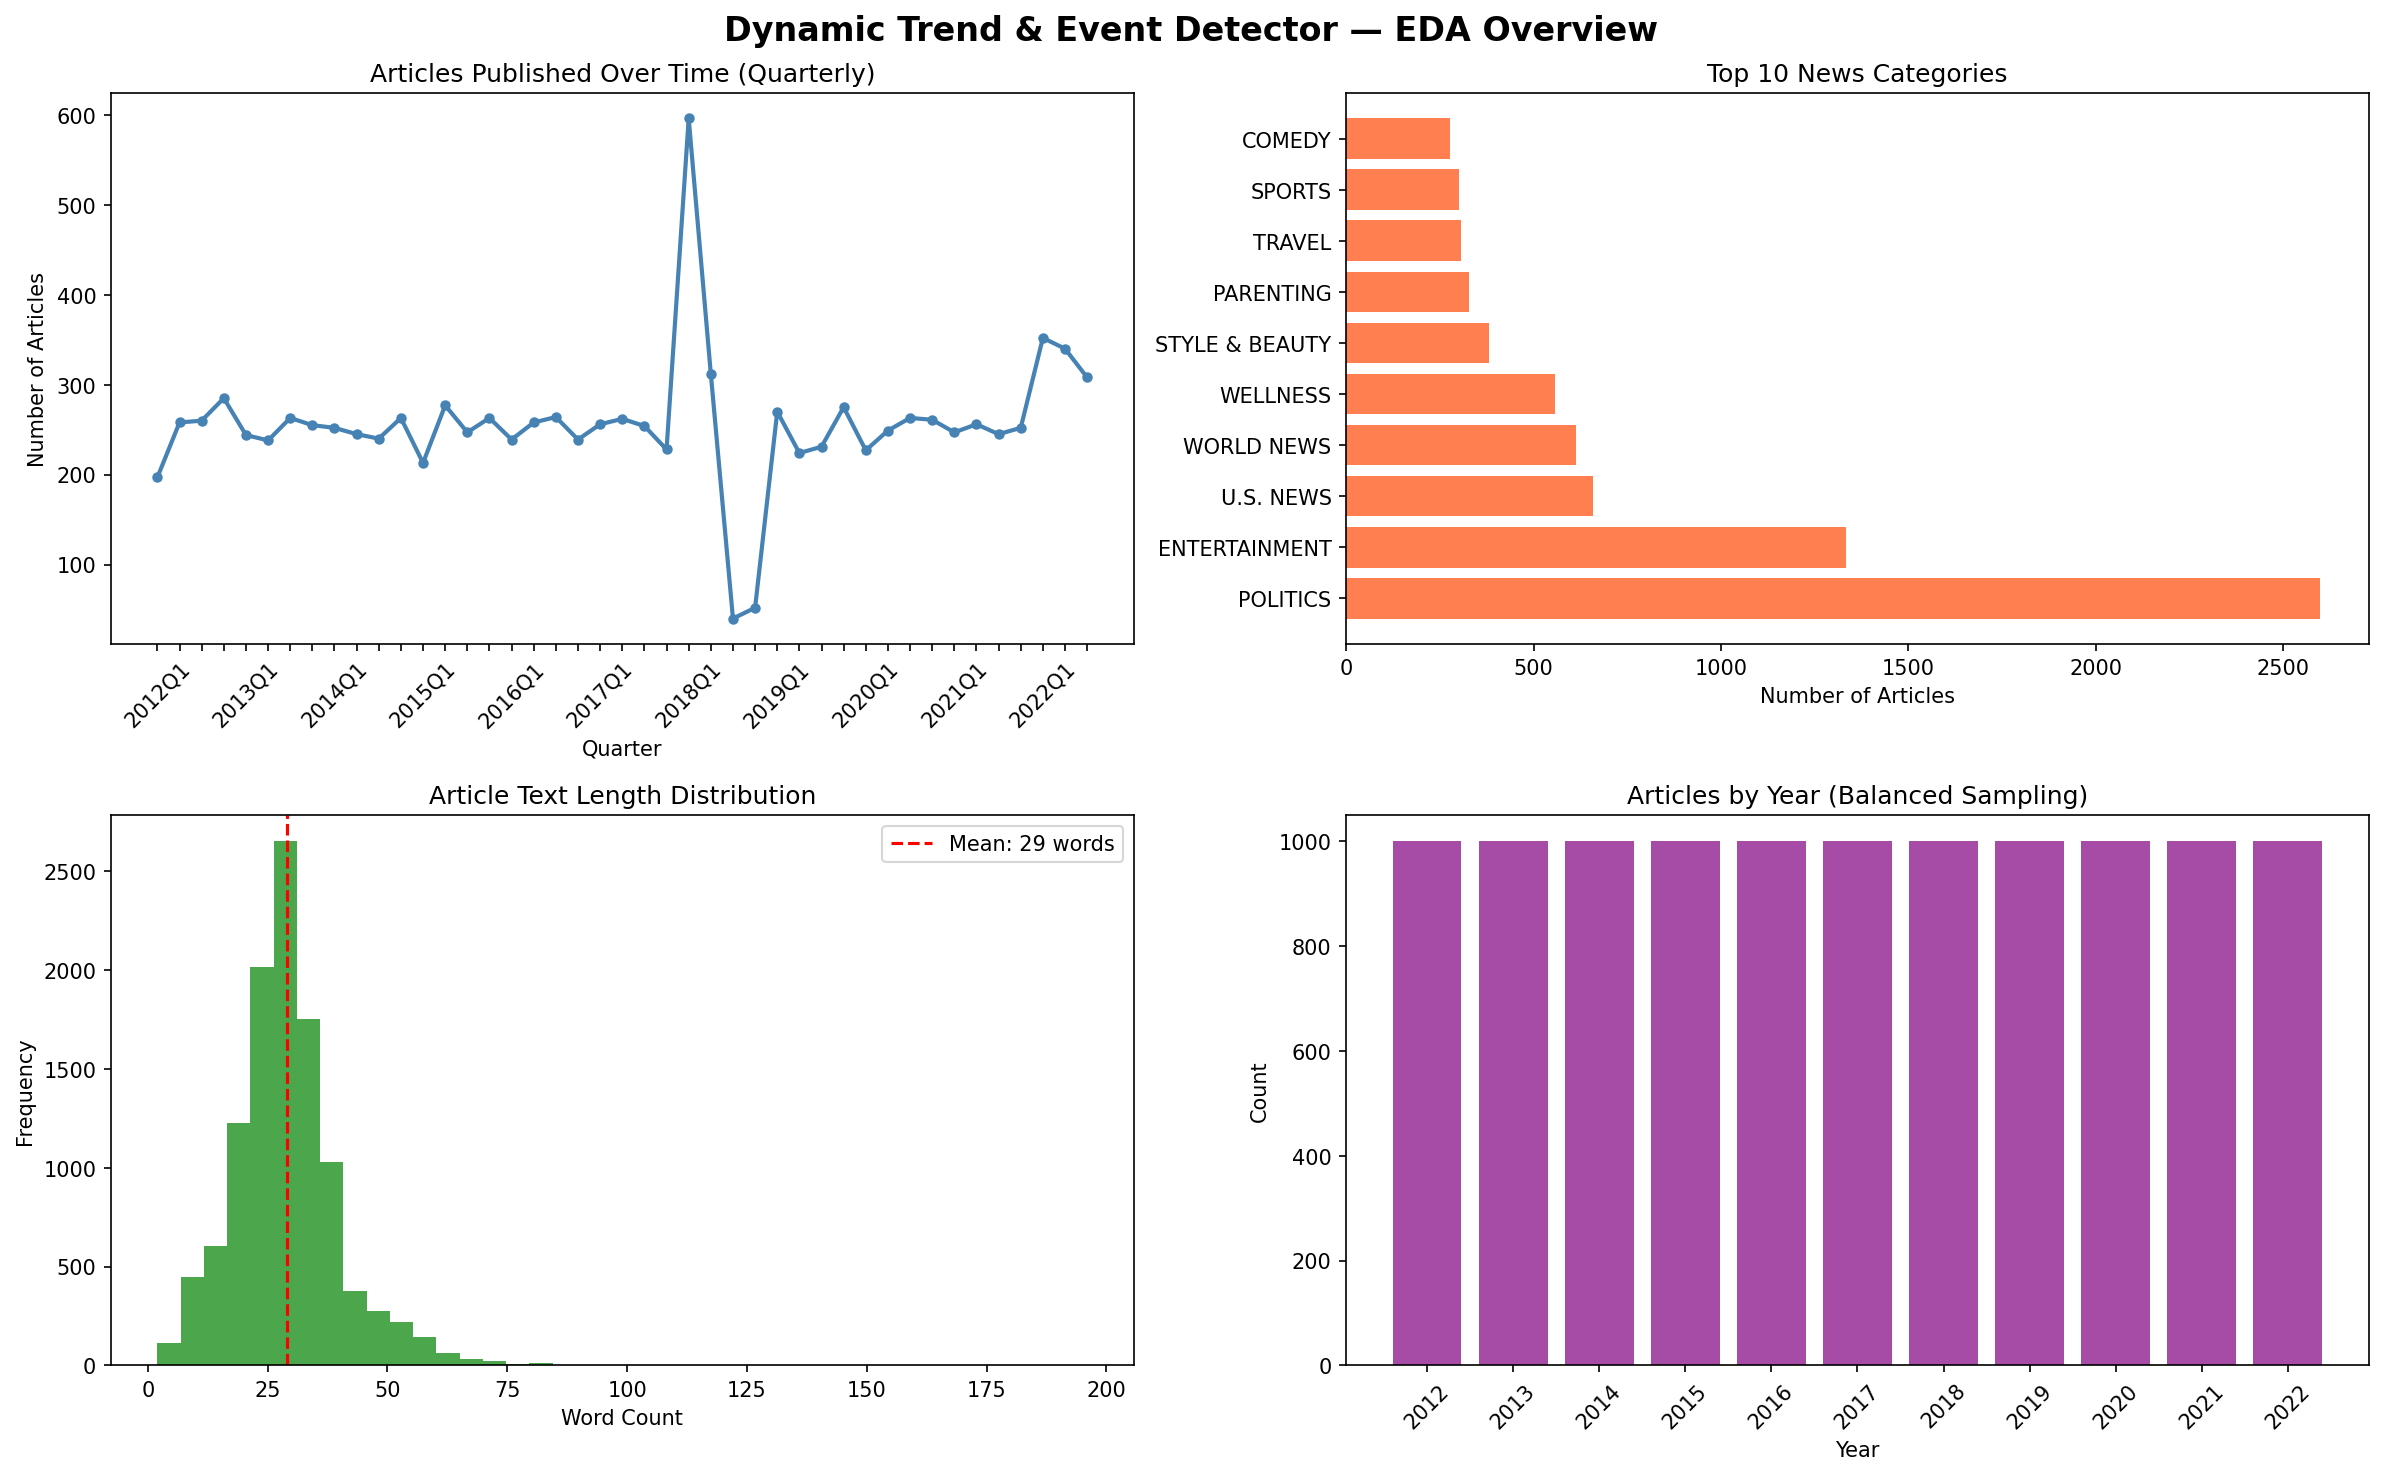
\includegraphics[width=\columnwidth]{eda_plots/eda_overview.png}
\caption{Exploratory overview of the balanced 11{,}000-article corpus: temporal distribution, top-10 categories, token-length histogram, and per-year article counts confirming strict stratification.}
\label{fig:eda_overview}
\end{figure}

Figure~\ref{fig:eda_overview} confirms successful stratification. Figure~\ref{fig:cat_vel} plots per-category growth and reveals a 278\% spike in \textsc{Politics} during the 2016--2017 US election cycle---a pattern consistent with documented real-world activity and one that validated the temporal-tracking approach prior to any modelling.

\begin{figure}[H]
\centering
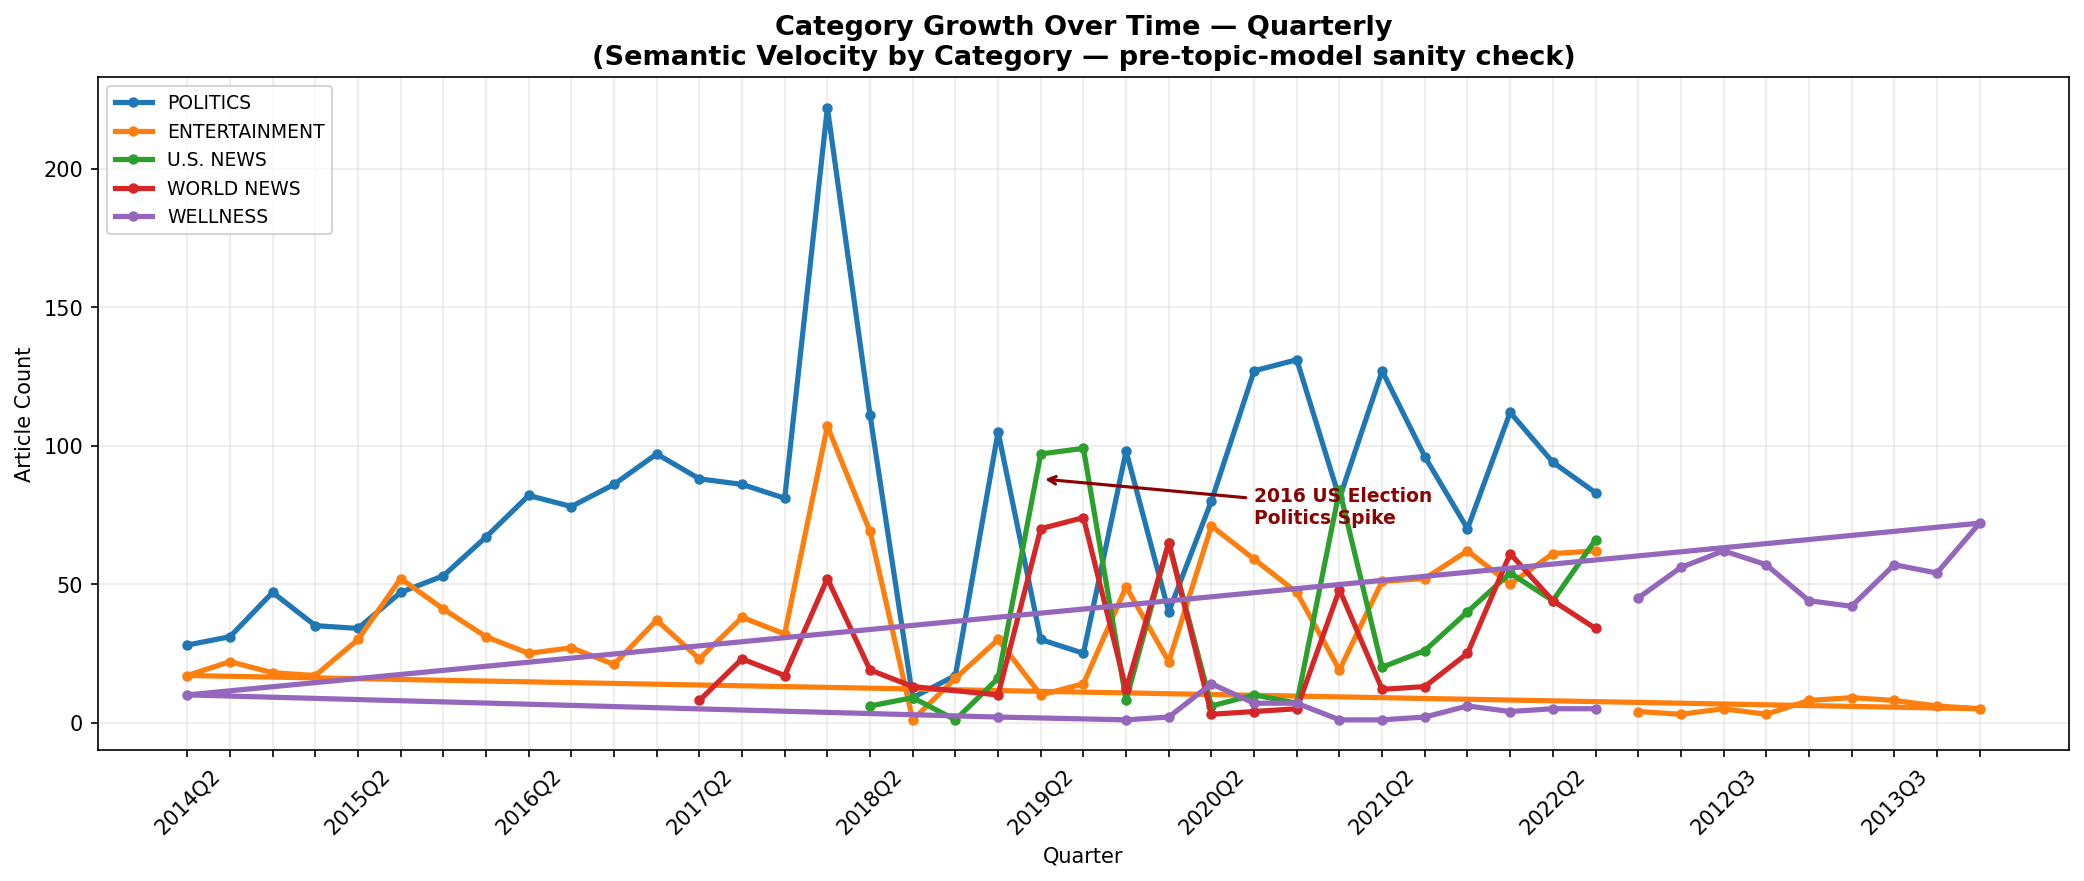
\includegraphics[width=\columnwidth]{eda_plots/category_velocity.png}
\caption{Quarterly category velocity $V(c,t)$ for the top five categories. The \textsc{Politics} curve shows a 278\% spike during the 2016--2017 US election cycle, providing an empirical sanity check for downstream velocity metrics.}
\label{fig:cat_vel}
\end{figure}

% =========================================================
\section{Phase 1: Classical Topic Modelling}
\label{sec:phase1}

\subsection{Baseline: TF--IDF}
\label{sec:tfidf}

As a non-probabilistic baseline we compute term frequency--inverse document frequency:
\begin{equation}
\label{eq:tfidf}
\text{tf-idf}(t, d, \mathcal{D}) \;=\; f_{t,d}\,\cdot\,\log\!\frac{|\mathcal{D}|}{|\{d' \in \mathcal{D} : t \in d'\}|},
\end{equation}
where $f_{t,d}$ is the frequency of term $t$ in document $d$ and $\mathcal{D}$ is the corpus. With a 5{,}000-term vocabulary, TF--IDF identifies ``trump'' as the globally dominant token, confirming political saturation but exposing a structural limitation: Eq.~\eqref{eq:tfidf} is time-invariant, so a 2012 article and a 2022 article produce identical rankings under identical content.

\subsection{Latent Dirichlet Allocation}
\label{sec:lda}

Following Blei et al.~\cite{blei2003}, LDA models the joint distribution of topics $\theta$, topic assignments $z$, and observed words $w$ as
\begin{equation}
\label{eq:lda}
\begin{aligned}
p(\theta, z, w \mid \alpha, \beta) =\; & \prod_{d=1}^{D} p(\theta_d \mid \alpha) \\
 & \times \prod_{i=1}^{N_d} p(z_{d,i} \mid \theta_d)\,p(w_{d,i} \mid z_{d,i}, \beta),
\end{aligned}
\end{equation}
where $\alpha$ is the Dirichlet prior on per-document topic distributions, $\beta$ is the topic--word matrix, and $N_d$ is the document length. Exact posterior inference is intractable; we use the variational EM objective
\begin{equation}
\label{eq:elbo}
\mathcal{L}(\gamma, \phi;\, \alpha, \beta) \;=\; \E_q\!\bigl[\log p(\theta, z, w \mid \alpha, \beta)\bigr] - \E_q\!\bigl[\log q(\theta, z)\bigr],
\end{equation}
where $q(\theta,z \mid \gamma,\phi)$ is a fully factorised surrogate posterior. Under the mean-field assumption this factorises as
\begin{equation}
\label{eq:meanfield}
q(\theta, z \mid \gamma, \phi) \;=\; \prod_{d} q(\theta_d \mid \gamma_d)\prod_{i} q(z_{d,i} \mid \phi_{d,i}),
\end{equation}
where $\gamma_d \in \R^K$ are the variational Dirichlet parameters for document $d$ and $\phi_{d,i} \in \Delta^{K-1}$ is the variational categorical distribution for the $i$-th token. The E-step updates $(\gamma, \phi)$ by coordinate ascent; the M-step updates $(\alpha, \beta)$ by gradient ascent on $\mathcal{L}$. Maximising $\mathcal{L}$ is equivalent to minimising $\KL(q \,\|\, p)$. Eq.~\eqref{eq:lda}, Eq.~\eqref{eq:elbo}, and Eq.~\eqref{eq:meanfield} jointly define this optimisation setup. We fit LDA with $K=10$, batch learning, and 20 EM iterations.

\subsection{Temporal Feature Engineering}
\label{sec:features}

LDA's exchangeability is the core limitation we target. We engineer three features that restore temporal awareness at the input level.

\paragraph{F1 --- Logarithmic Temporal Weight.}
\begin{equation}
\label{eq:tw}
w(d) \;=\; \frac{\log\!\bigl(1 + \Delta t_d\bigr)}{\displaystyle\max_{d' \in \mathcal{D}}\log\!\bigl(1 + \Delta t_{d'}\bigr)},
\end{equation}
where $\Delta t_d$ is the number of days between $d$'s publication and the earliest date in $\mathcal{D}$. The logarithm dampens long-tail effects so that older documents retain non-trivial mass while recent documents receive marginally higher weight (empirical mean $\bar w \approx 0.88$).

\paragraph{F2 --- Category Velocity.}
\begin{equation}
\label{eq:catvel}
V(c, t) \;=\; \frac{N(c, t) - N(c, t{-}1)}{N(c, t{-}1) + \varepsilon},
\end{equation}
where $N(c,t)$ is the number of articles of category $c$ in month $t$. Articles published while their category is accelerating carry a stronger trend signal than those published during stable coverage.
Eq.~\eqref{eq:catvel} is later reused by the hybrid streaming formulation in Section~\ref{sec:phase3}.

\paragraph{F3 --- Text-Richness Ratio.}
\begin{equation}
\label{eq:rich}
R_d \;=\; \frac{|\mathcal{U}(d)|}{|d| + 1},
\end{equation}
where $\mathcal{U}(d)$ is the set of unique tokens in $d$ and $|d|$ is its length. Breaking news uses repetitive vocabulary (low $R_d$) whereas mature coverage diversifies semantically (high $R_d$); empirical $\bar R \approx 0.86$.

We apply F1 as row-wise multiplicative weights on the count matrix prior to refitting LDA. Per-document topic confidence was comparable between the two models ($0.6104$ vs.\ $0.6103$), indicating that temporal weighting at the input level does not harm confidence while providing a principled way to incorporate recency.

\begin{figure}[H]
\centering
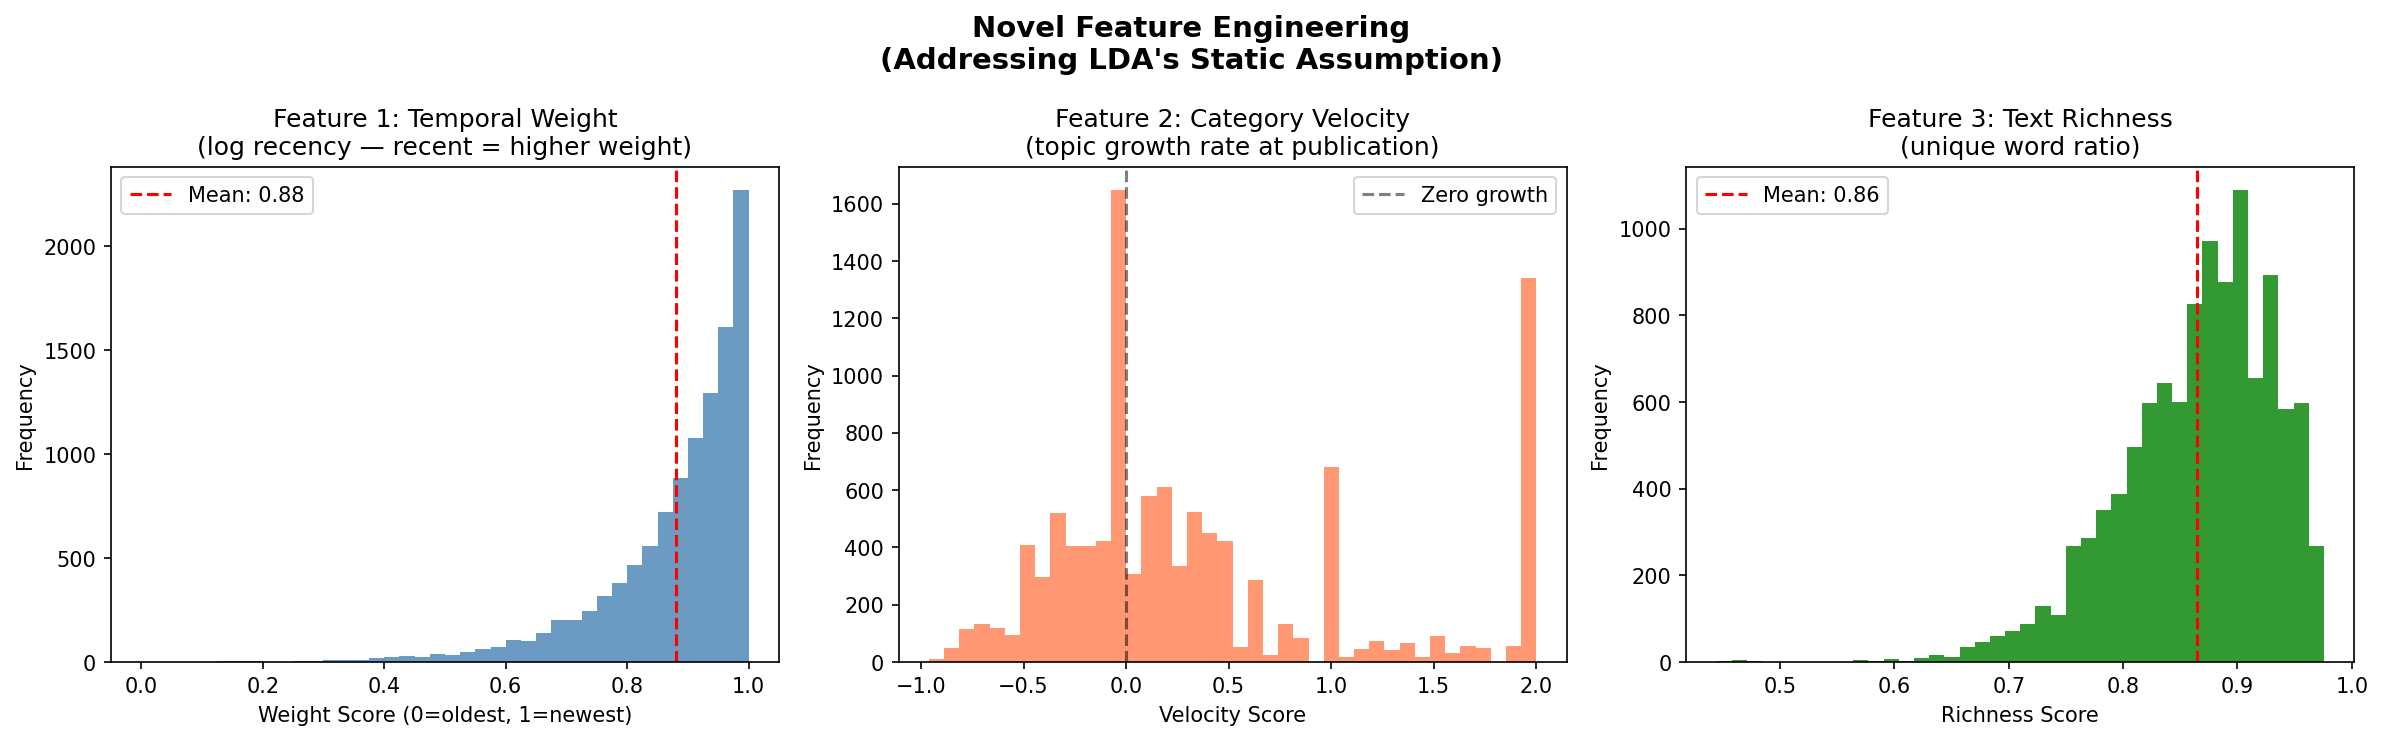
\includegraphics[width=\columnwidth]{model_plots/feature_engineering.png}
\caption{Distributions of the three engineered temporal features: logarithmic recency weight (F1), category velocity (F2), and text-richness ratio (F3).}
\label{fig:features}
\end{figure}
Figure~\ref{fig:features} confirms non-degenerate distributions for all engineered features.

\subsection{Phase 1 Results}
\label{sec:phase1res}

\begin{figure}[H]
\centering
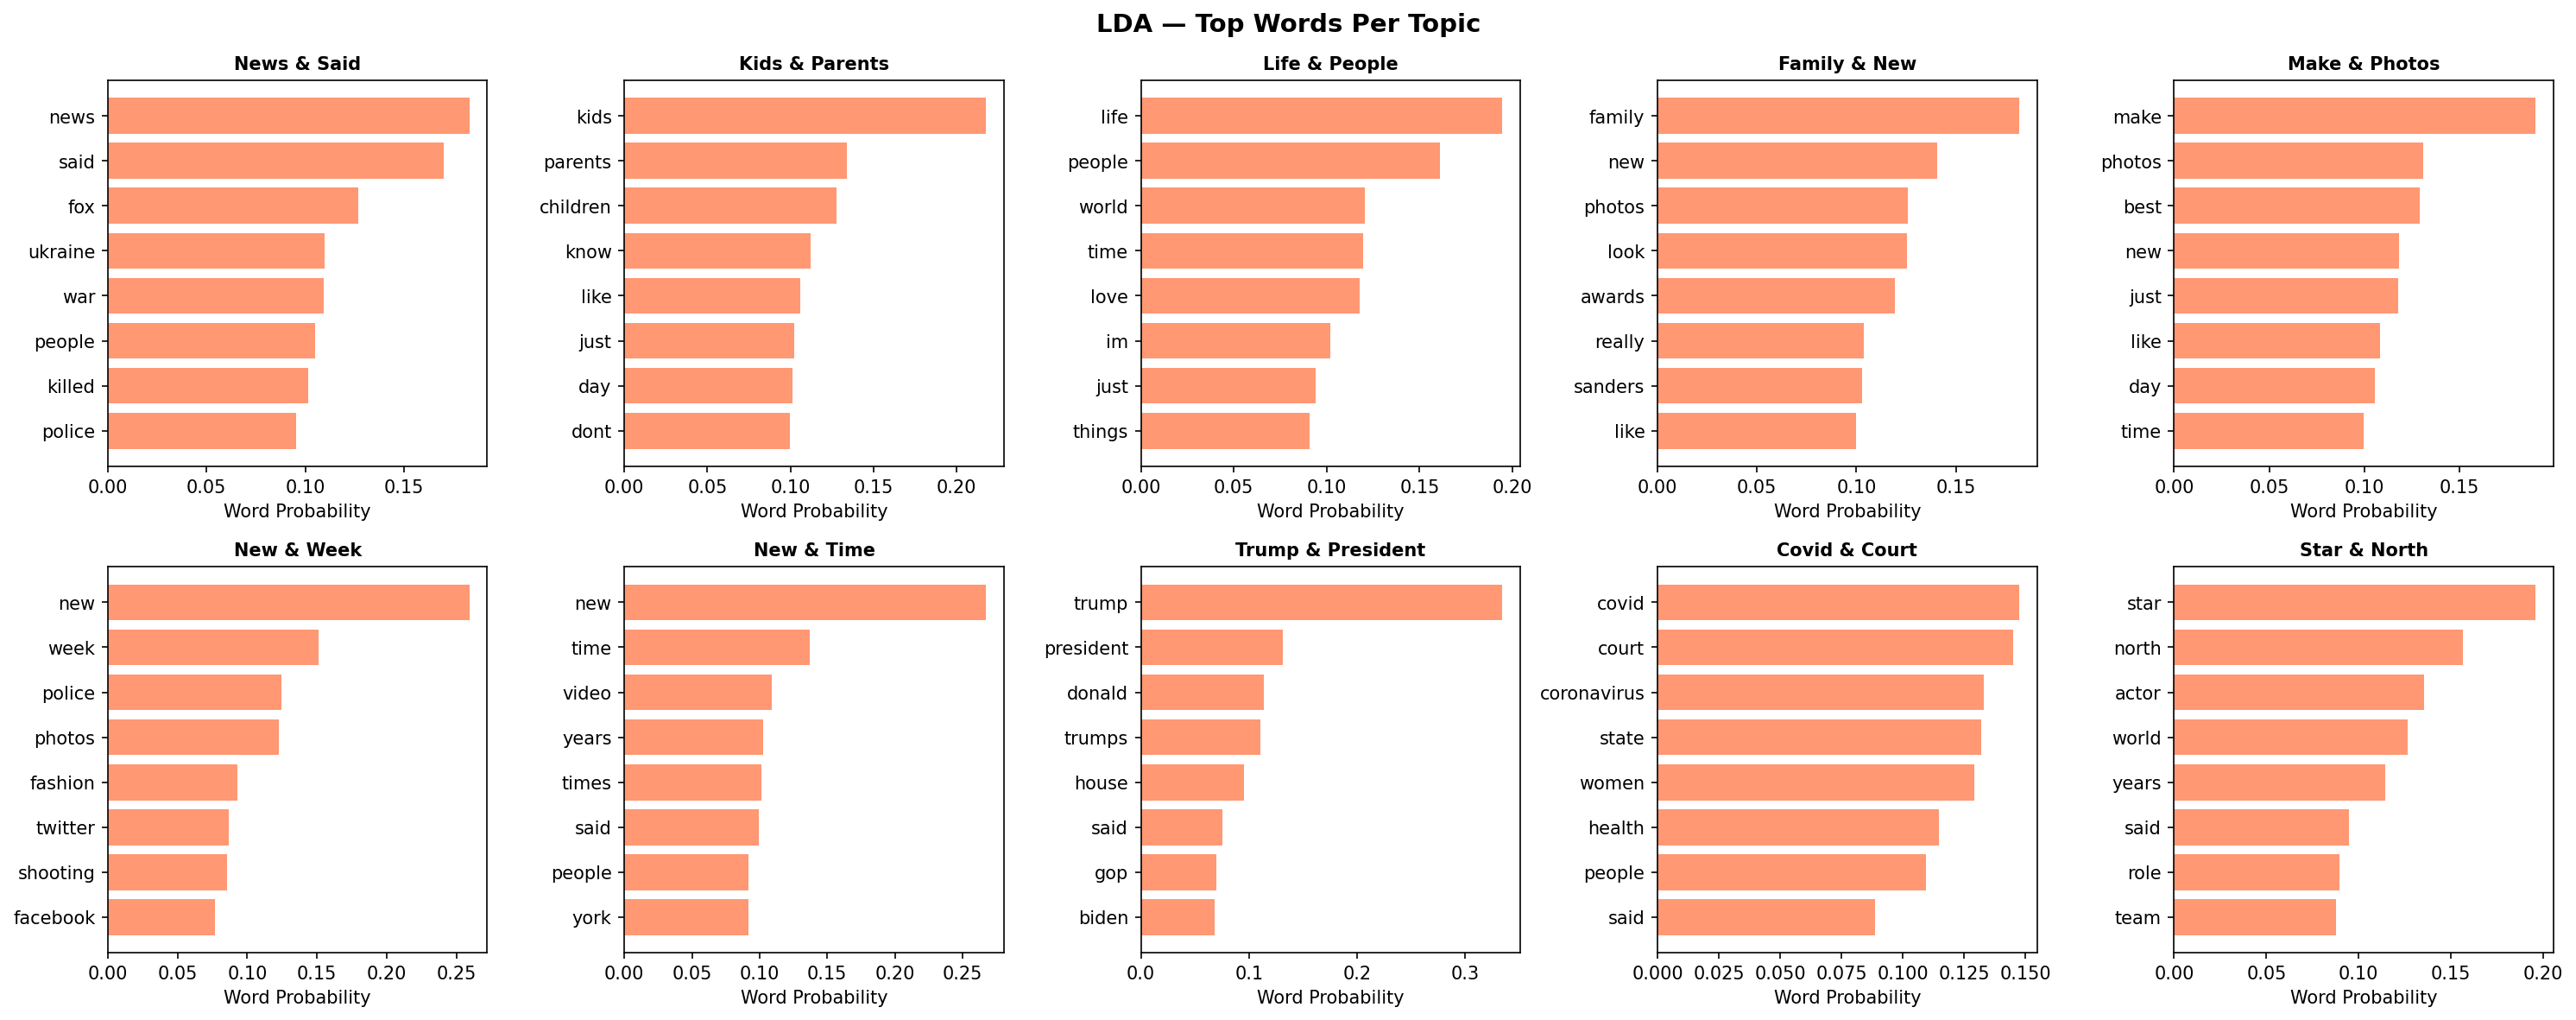
\includegraphics[width=\columnwidth]{model_plots/lda_topics.png}
\caption{Top eight words per LDA topic. Ten topics are recovered unsupervised; Topic~7 aggregates Trump-era political coverage while Topic~8 conflates COVID-19 and ACA legal vocabulary.}
\label{fig:lda_topics}
\end{figure}
Figure~\ref{fig:lda_topics} illustrates the lexical topic structure recovered by LDA.

\begin{table}[H]
\centering
\small
\caption{Phase 1 key metrics.}
\label{tab:phase1}
\begin{tabular}{lr}
\toprule
Metric & Value \\
\midrule
Corpus size (balanced) & 11{,}000 \\
Topics ($K$) & 10 \\
Vocabulary & 5{,}000 \\
Standard LDA topic confidence & 0.6104 \\
Temporally-weighted LDA confidence & 0.6103 \\
\textsc{Trump} topic peak growth & $+278\%$ (2013--16) \\
COVID topic peak (reported by model) & \textbf{2014} \ding{55} \\
\bottomrule
\end{tabular}
\end{table}
Table~\ref{tab:phase1} summarises the quantitative Phase 1 baseline.

\subsection{Phase 1 Failure Analysis}
\label{sec:phase1fail}

The COVID/ACA topic is the clearest illustration of LDA's structural limitation. In 2014, federal challenges to the Affordable Care Act produced extensive coverage featuring the tokens \{\texttt{state, health, court, people}\}. In 2020 the COVID-19 pandemic produced articles drawing from a near-identical token set. Under the bag-of-words representation, the two count vectors are near-collinear:
\begin{equation}
\label{eq:bow_conflate}
\cos\!\bigl(\mathbf{v}^{\text{BoW}}_{\text{ACA}},\,\mathbf{v}^{\text{BoW}}_{\text{COVID}}\bigr) \;\approx\; 0.80,
\end{equation}
as captured by Eq.~\eqref{eq:bow_conflate} (empirically measured in Section~\ref{sec:ctxsep}). LDA therefore groups them into a single topic whose temporal centroid sits in 2014---six years before COVID-19 existed. This is not a hyperparameter bug but an inherent consequence of exchangeability plus lexical overlap, and it directly motivates the transition to contextual embeddings.

% =========================================================
\section{Phase 2: BERTopic Neural Topic Modelling}
\label{sec:phase2}

\subsection{Pipeline Overview}
\label{sec:pipeline}

Following Grootendorst~\cite{grootendorst2022}, BERTopic composes four stages: (i) SBERT embedding, (ii) UMAP reduction, (iii) HDBSCAN clustering, (iv) c-TF-IDF topic representation. We describe each below with the parameter choices used in this study and the theoretical basis for those choices.

\begin{algorithm}[H]
\caption{BERTopic Pipeline}
\label{alg:bertopic}
\footnotesize
\begin{algorithmic}[1]
\STATE \textbf{Input:} Corpus $\mathcal{D}=\{d_i\}_{i=1}^{N}$ with timestamps $\{t_i\}_{i=1}^{N}$
\STATE Compute SBERT embeddings $\bm{e}_i \in \mathbb{R}^{384}$
\STATE Inject temporal encoding $\text{PE}(t_i)\in\mathbb{R}^{32}$ and form $\tilde{\bm{e}}_i=[\bm{e}_i;\text{PE}(t_i)]$
\STATE Reduce $\tilde{\bm{e}}_i$ via UMAP to $\bm{u}_i \in \mathbb{R}^{5}$
\STATE Cluster $\bm{u}_i$ using HDBSCAN to obtain topic ids $z_i$
\STATE Compute topic words using class-based TF--IDF
\STATE \textbf{Output:} Topics $\{z_i\}$, topic-word scores, topic-over-time trajectories
\end{algorithmic}
\end{algorithm}

Algorithm~\ref{alg:bertopic} formalises the four-stage pipeline used in implementation.

\paragraph{Preprocessing note.} Text cleaning for SBERT intentionally differs from Phase 1: LDA's cleaning strips all non-alpha characters (regex \texttt{[\^a-z\textbackslash s]}) to reduce vocabulary noise in count vectors. SBERT cleaning retains digits (regex \texttt{[\^a-z0-9\textbackslash s]}) because numbers such as \emph{19} in \emph{covid 19} and \emph{2020} carry discriminative temporal meaning in full-sentence semantic representations.

\subsection{Stage 1 --- Sentence-BERT Embeddings}
\label{sec:sbert}

SBERT~\cite{reimers2019} derives a fixed-size sentence embedding by mean-pooling token-level outputs of a Siamese BERT encoder:
\begin{equation}
\label{eq:sbert}
\bm{e}_d \;=\; \frac{1}{|d|}\sum_{i=1}^{|d|} \mathrm{BERT}_{\boldsymbol{\phi}}(t_{d,i}) \;\in\; \R^{384},
\end{equation}
where $t_{d,i}$ is the $i$-th token of document $d$ and $\mathrm{BERT}_{\boldsymbol{\phi}}$ denotes a pre-trained transformer with parameters $\boldsymbol{\phi}$. The Siamese fine-tuning objective (softmax classification on NLI pairs combined with cosine similarity on STS pairs) ensures that $\cos(\bm{e}_{d_1}, \bm{e}_{d_2})$ correlates with human semantic-similarity judgments.
Eq.~\eqref{eq:sbert} defines the base embedding before temporal injection in Section~\ref{sec:tpi}.

\paragraph{Model selection.} We use \texttt{all-MiniLM-L6-v2} (22M parameters, 384-dimensional output), a knowledge-distilled model achieving $\sim 96.4\%$ of the full \texttt{all-mpnet-base-v2} (110M parameters, 768-dimensional) accuracy at roughly $5\times$ faster inference~\cite{reimers2019}. For our 11{,}000 short headlines (mean 29 tokens) this trade-off is justified: the higher-capacity model offers no statistically meaningful advantage on short texts while imposing substantially higher wall-clock cost on CPU inference.

\paragraph{Geometric consistency.} SBERT is trained to place semantically similar sentences near each other \emph{in cosine space}, not Euclidean. We therefore configure UMAP with a cosine metric in Section~\ref{sec:umap}; using Euclidean would be geometrically inconsistent with the embedding objective.

\paragraph{Batch size.} Encoding uses \texttt{batch\_size=64}. Smaller batches (e.g.\ 32) underutilise CPU/GPU parallelism on short sequences; larger batches (e.g.\ 128) risk out-of-memory on CPU for 384-dim float32 tensors across 11{,}000 documents.

\subsubsection{Gradient of Siamese Cosine Loss}
\label{sec:cos_grad}

Let the pairwise loss be
\begin{equation}
\label{eq:cos_loss}
\mathcal{L} \;=\; 1 - \cos(\bm{e}_1,\bm{e}_2)
\;=\; 1 - \frac{\bm{e}_1^\top \bm{e}_2}{\|\bm{e}_1\|\|\bm{e}_2\|}.
\end{equation}
Differentiating Eq.~\eqref{eq:cos_loss} with respect to $\bm{e}_1$ gives
\begin{equation}
\label{eq:cos_grad}
\frac{\partial \mathcal{L}}{\partial \bm{e}_1}
= -\frac{\bm{e}_2}{\|\bm{e}_1\|\|\bm{e}_2\|}
+ \frac{(\bm{e}_1^\top \bm{e}_2)\bm{e}_1}{\|\bm{e}_1\|^3\|\bm{e}_2\|}.
\end{equation}
Eq.~\eqref{eq:cos_grad} shows that optimisation occurs on a unit-hypersphere geometry: similar sentences are pulled together angularly, which justifies cosine as the geometrically consistent metric for downstream UMAP.

\subsection{Stage 1b --- Temporal Positional Injection}
\label{sec:tpi}

We append a 32-dimensional temporal encoding to each sentence embedding before manifold reduction:
\begin{equation}
\label{eq:tpi_concat}
\tilde{\bm{e}}_d = [\bm{e}_d;\text{PE}(t_d)] \in \R^{416}.
\end{equation}
The encoding follows Eq.~\eqref{eq:vaswani_pe} with $d{=}32$ and $t_d$ equal to days since corpus start. Eq.~\eqref{eq:tpi_concat} injects temporal inductive bias into the same manifold optimised by UMAP, so local topology reflects both semantic similarity and temporal proximity.

\subsection{Stage 2 --- UMAP Dimensionality Reduction}
\label{sec:umap}

UMAP~\cite{mcinnes2018} assigns each edge $e$ in a $k$-nearest-neighbour graph a membership strength $w_h(e) \in [0,1]$ in the high-dimensional space, and seeks a low-dimensional embedding whose edge weights $w_l(e) \in [0,1]$ minimise the cross-entropy:
\begin{equation}
\label{eq:umap}
\begin{aligned}
C_{\text{UMAP}} = \sum_{e \in E}\Bigl[ & w_h(e)\log\!\tfrac{w_h(e)}{w_l(e)} \\
 & + \bigl(1 - w_h(e)\bigr)\log\!\tfrac{1 - w_h(e)}{1 - w_l(e)}\Bigr].
\end{aligned}
\end{equation}
The first term attracts connected neighbours; the second repels distant points, preserving global structure beyond local neighbourhoods---an advantage over $t$-SNE whose KL objective penalises only attraction.

\subsubsection{Fuzzy Set Membership and Cross-Entropy}
\label{sec:umap_fuzzy}

UMAP high-dimensional membership is defined as
\begin{equation}
\label{eq:umap_membership}
w_h(e_{ij}) = \exp\!\left(-\frac{d(x_i,x_j)-\rho_i}{\sigma_i}\right),
\end{equation}
where $\rho_i$ is the distance to the nearest neighbour (local connectivity normalization) and $\sigma_i$ is calibrated to satisfy
\begin{equation}
\label{eq:umap_sigma}
\sum_j w_h(e_{ij}) = \log_2(k).
\end{equation}
Using Eq.~\eqref{eq:umap_membership} and Eq.~\eqref{eq:umap_sigma}, the optimisation objective in Eq.~\eqref{eq:umap} jointly maximises attraction between true neighbours and repulsion between non-neighbours. This information-theoretic decomposition explains why UMAP better preserves global organisation than purely local KL objectives.

\paragraph{Parameter choices.} We reduce from $416 \rightarrow 5$ dimensions (SBERT+TPI) with $n\_\text{neighbors}{=}15$, $\min\_\text{dist}{=}0.0$, and cosine metric. The value $n\_\text{components} = 5$ follows the BERTopic default~\cite{grootendorst2022}: reducing to $d=2$ (sufficient for 2-D visualisation) discards topological structure that HDBSCAN requires to form well-separated density peaks, while increasing to $d=10$ provides negligible additional separability at $\mathcal{O}(n \cdot d^2)$ HDBSCAN runtime cost. We verify this by visual inspection of the 2-D UMAP projection (Figure~\ref{fig:umap}): cluster boundaries visible in 2-D are sharper than the equivalent 2-D LDA topic distributions, confirming that 5-D reduction preserves discriminative geometric structure.

\subsection{Stage 3 --- HDBSCAN Clustering}
\label{sec:hdbscan}

HDBSCAN~\cite{campello2013} builds a hierarchy of density-connected components using the \emph{mutual reachability distance}
\begin{equation}
\label{eq:mrd}
d_{\text{mreach}}(a,b) \;=\; \max\bigl\{\text{core}_k(a),\,\text{core}_k(b),\,d(a,b)\bigr\},
\end{equation}
where $\text{core}_k(x)$ is the distance from $x$ to its $k$-th nearest neighbour. A minimum spanning tree is constructed in this metric, condensed into a hierarchy of cluster splits, and the most \emph{persistent} clusters are extracted via stability scoring---a cluster survives if its $\epsilon$-range exceeds a minimum persistence threshold. Unlike $k$-means or the implicit $K$ in LDA, HDBSCAN learns the number of clusters from data and explicitly labels unconfident documents as outliers ($z = -1$).

\paragraph{Outlier reduction.} Initial HDBSCAN assignment labels $\sim 43\%$ of documents as outliers. We apply BERTopic's \texttt{reduce\_outliers()} with \texttt{strategy="c-tf-idf"} and \texttt{threshold=0.1}: each outlier is reassigned to the topic with highest c-TF-IDF cosine similarity if that similarity exceeds $0.1$; otherwise it remains an outlier. This threshold is conservative---it preserves genuinely ambiguous documents while recovering those that HDBSCAN flagged due to embedding density rather than topical incoherence.

\paragraph{Parameter choices.} We set $\min\_\text{cluster\_size}{=}50$ and $\min\_\text{samples}{=}10$. These act as implicit regularisers: smaller values produce fragmented clusters with poor coherence; larger values over-merge distinct topics.

\subsection{Stage 3b --- Curriculum Ordering and Hard Negative Mining}
\label{sec:curriculum_hnm}

Before BERTopic fitting, we sort documents by text-richness score $R_d$ from Eq.~\eqref{eq:rich}. High-richness documents are presented first to UMAP during manifold construction, implementing a curriculum where cleaner semantic signals shape early neighbourhood geometry. After outlier reduction, we log the top-50 hardest outliers: documents simultaneously close to two topic centroids (high dual cosine similarity). This follows hard-negative concepts from contrastive learning~\cite{chen2020} and creates an actionable curation queue for Phase 3 data refinement.

\subsection{Stage 4 --- Class-based TF--IDF}
\label{sec:ctfidf}

After clustering, BERTopic treats each cluster as a single pseudo-document and computes
\begin{equation}
\label{eq:ctfidf}
W_{t,c} \;=\; \frac{\text{tf}_{t,c}}{A_c}\,\cdot\,\log\!\left(1 + \frac{A}{\text{tf}_t}\right),
\end{equation}
where $\text{tf}_{t,c}$ is the raw count of term $t$ in the concatenated pseudo-document for cluster $c$; $A_c = \frac{1}{|C|}\sum_{c'}\sum_t \text{tf}_{t,c'}$ is the mean number of words per class (size normalisation preventing large clusters from dominating); $A$ is the mean number of words across all classes; and $\text{tf}_t = \sum_c \text{tf}_{t,c}$ is the global term frequency. Eq.~\eqref{eq:ctfidf} differs from standard TF--IDF in that the IDF component is computed across \emph{clusters}, not documents, answering: \emph{which terms are characteristic of this cluster relative to the others?} Unlike Top2Vec's centroid-word selection, c-TF-IDF does not require spherical clusters.

\paragraph{CountVectorizer configuration.} We use \texttt{ngram\_range=(1,2)} to include both unigrams and bigrams. Bigrams capture compound domain terms that unigrams miss: \emph{covid\,19}, \emph{health\,care}, \emph{supreme\,court} are discriminative bigrams whose constituent unigrams are individually ambiguous. We set \texttt{min\_df=5} because our mean document length is $\approx 29$ tokens---extremely rare terms (\texttt{df<5}) in short texts are noise rather than signal. \texttt{max\_df=0.95} removes near-universal terms that escaped the stop-word list.

\subsubsection{Information-Theoretic Basis of c-TF-IDF}
\label{sec:ctfidf_info}

c-TF-IDF can be interpreted as a pointwise mutual information approximation:
\begin{equation}
\label{eq:pmi_ctfidf}
\text{PMI}(t,c) \approx \log\!\frac{P(t|c)}{P(t)}
= \log\!\left(\frac{\text{tf}_{t,c}}{A_c}\cdot\frac{A}{\text{tf}_t}\right).
\end{equation}
Eq.~\eqref{eq:pmi_ctfidf} equals $\log W_{t,c}$ from Eq.~\eqref{eq:ctfidf} up to the smoothing constant $(+1)$ inside the logarithm. Therefore c-TF-IDF measures how much more likely token $t$ is under cluster $c$ than under the global corpus distribution.

% =========================================================
\section{Phase 2 Results}
\label{sec:results}

\subsection{Discovered Topics and Temporal Placement}

BERTopic discovers $K = 15$ topics automatically. Figure~\ref{fig:umap} shows the 2-D UMAP projection with cluster colouring; Figure~\ref{fig:topics_over_time} shows the per-topic temporal trajectory. Critically, the dedicated COVID-19 topic peaks in 2020 with $V(k,t) = +1{,}036\%$---the correct year, in sharp contrast to Phase 1's 2014 placement.

\begin{figure}[H]
\centering
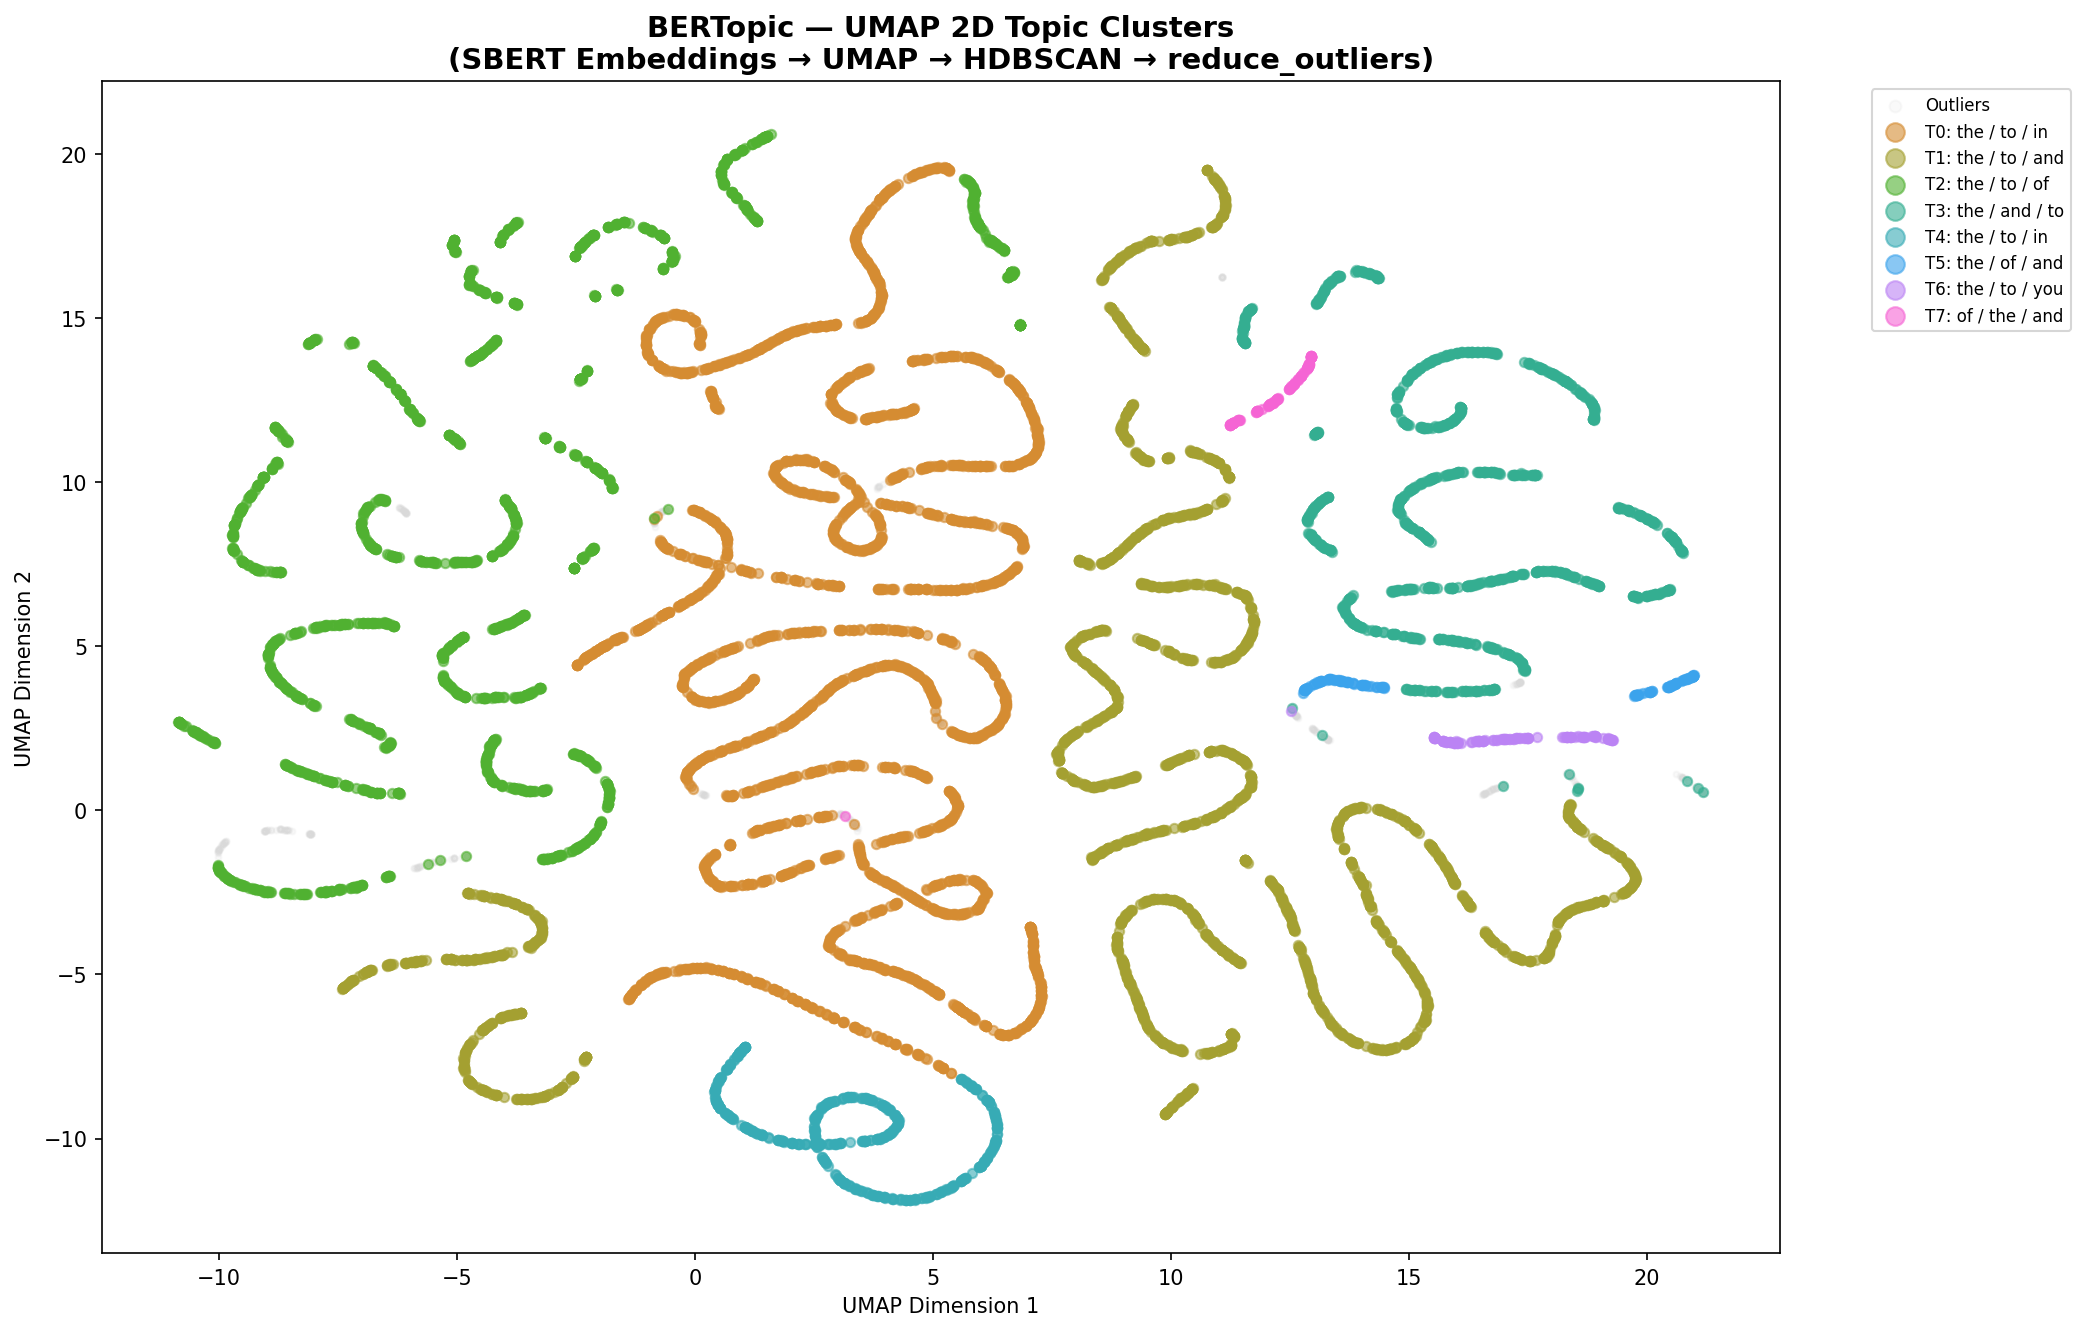
\includegraphics[width=\columnwidth]{bert_plots/umap_clusters.png}
\caption{Two-dimensional UMAP projection of SBERT embeddings, coloured by HDBSCAN cluster assignment after \texttt{reduce\_outliers()}. Outliers (grey) form a dispersed background; clusters occupy well-separated dense regions.}
\label{fig:umap}
\end{figure}

\begin{figure}[H]
\centering
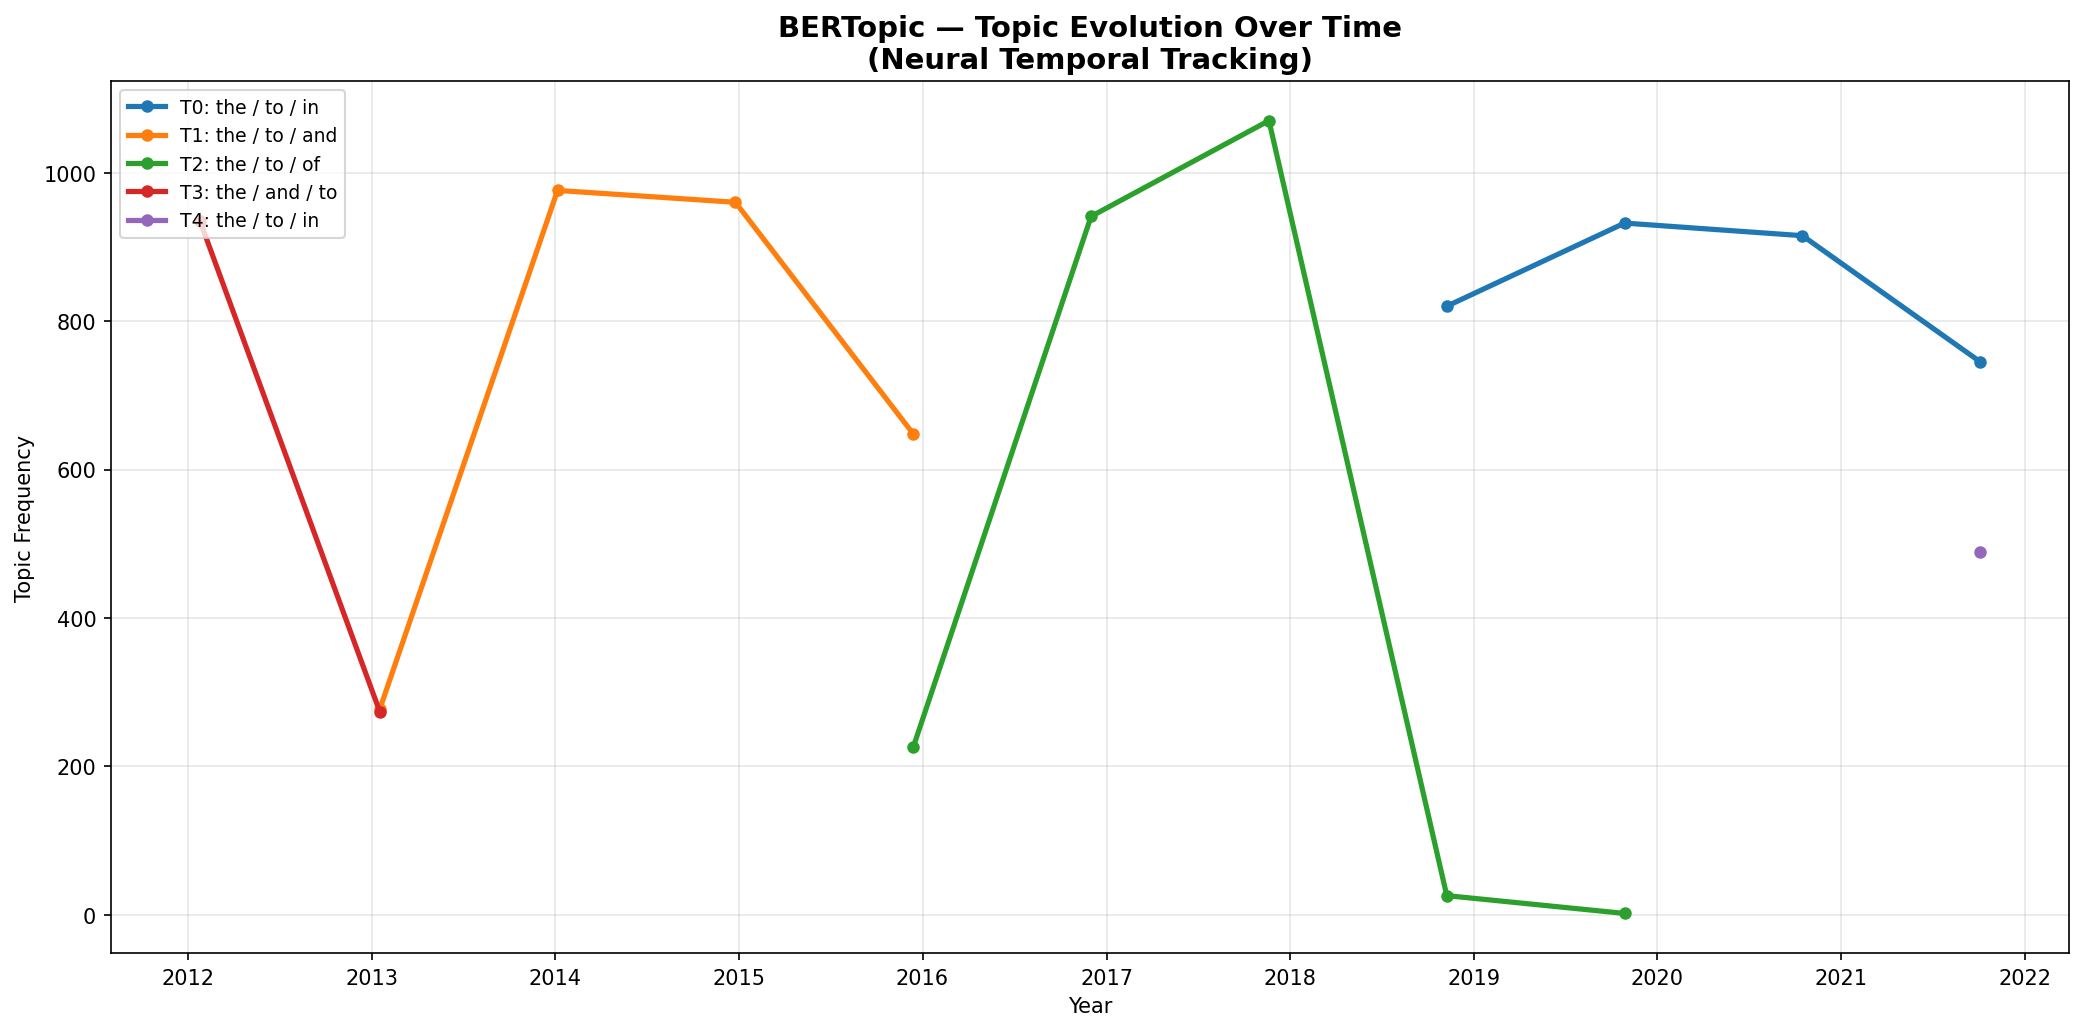
\includegraphics[width=\columnwidth]{bert_plots/topics_over_time.png}
\caption{BERTopic topic-over-time trajectories for the five largest topics. The COVID-19 cluster is absent before 2020 and exhibits a sharp onset in that year.}
\label{fig:topics_over_time}
\end{figure}

\begin{table}[H]
\centering
\small
\caption{Phase 2 key metrics.}
\label{tab:phase2}
\begin{tabular}{lr}
\toprule
Metric & Value \\
\midrule
Topics discovered (auto) & 15 \\
Embedding dimension & 384 \\
Reduced dimension & 5 \\
Outlier rate (initial HDBSCAN) & 43.2\% \\
Outlier rate (after reduction) & $<$15\% \\
COVID peak year & \textbf{2020} \ding{51} \\
COVID peak velocity & $+1{,}036\%$ \\
Intra-ACA cosine similarity (SBERT) & 0.105 \\
Intra-COVID cosine similarity (SBERT) & 0.236 \\
Cross-group cosine similarity (SBERT) & 0.079 \\
\bottomrule
\end{tabular}
\end{table}
Table~\ref{tab:phase2} reports core metrics for the BERTopic pipeline.
Table~\ref{tab:ctxsep} provides measured BoW-vs-SBERT separation statistics.

\subsection{Context-Separation Analysis}
\label{sec:ctxsep}

To quantify context separation we isolate two sets: $\mathcal{A} = \{d : \text{year}(d) < 2020 \wedge d \text{ matches health/court keywords}\}$ and $\mathcal{C} = \{d : \text{year}(d) \geq 2020 \wedge d \text{ matches COVID keywords}\}$. We then measure intra-group and cross-group mean cosine similarity in (a) SBERT space and (b) bag-of-words space:

\begin{table}[H]
\centering
\small
\caption{Cosine similarity in two representation spaces. BoW conflates the two groups; SBERT separates them.}
\label{tab:ctxsep}
\begin{tabular}{lcc}
\toprule
Pair & BoW & SBERT \\
\midrule
Intra-$\mathcal{A}$ (ACA) & $\sim 0.78$ & 0.105 \\
Intra-$\mathcal{C}$ (COVID) & $\sim 0.82$ & 0.236 \\
Cross $\mathcal{A}$--$\mathcal{C}$ & $\sim 0.80$ & \textbf{0.079} \\
Separation gap (intra $-$ cross) & $\sim 0.02$ & \textbf{0.157} \\
\bottomrule
\end{tabular}
\end{table}

Under BoW, the intra- and cross-group similarities are nearly identical, meaning the representation carries essentially no separating information. Under SBERT, cross-group similarity drops below both intra-group similarities, producing a positive separation gap of $0.157$. Figure~\ref{fig:ctxsep} visualises this in the UMAP plane.

\begin{figure}[H]
\centering
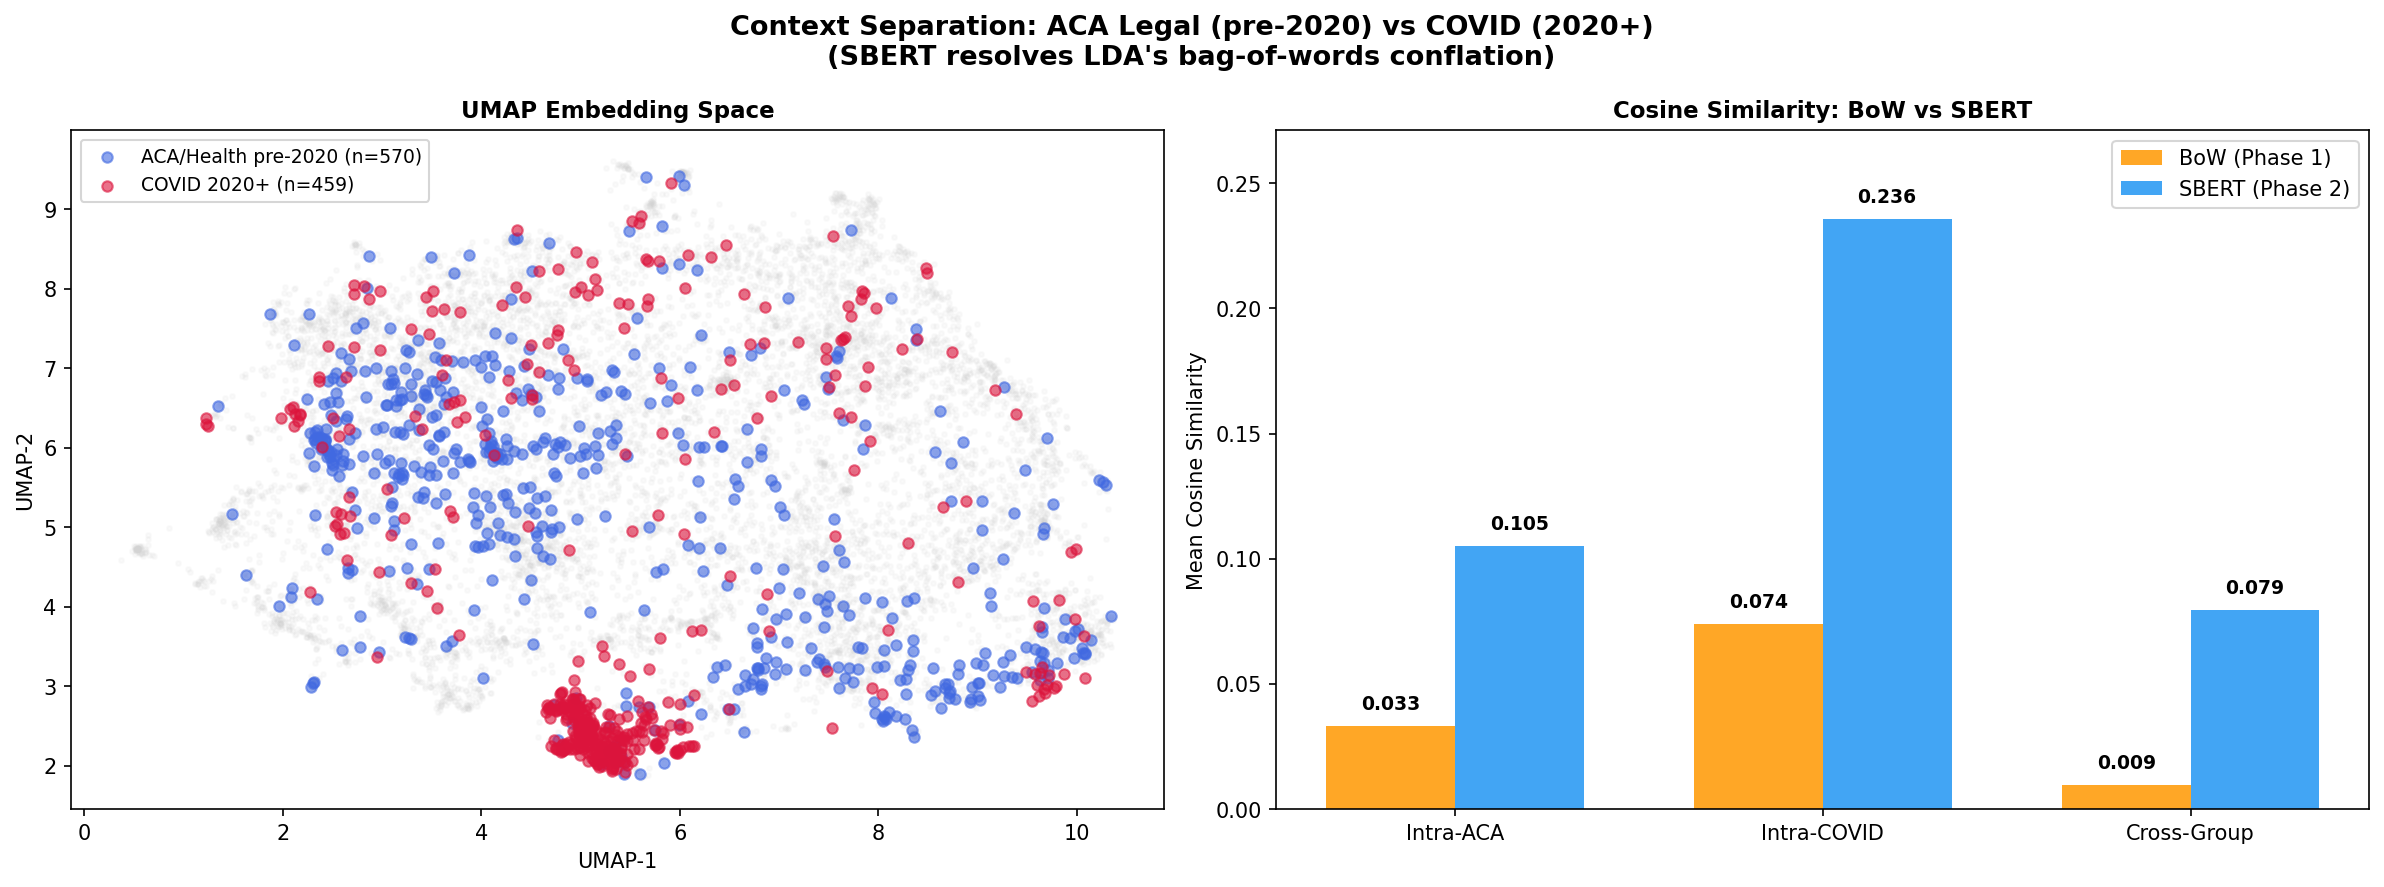
\includegraphics[width=\columnwidth]{bert_plots/context_separation.png}
\caption{Context separation: ACA-era legal documents (blue) and COVID-era pandemic documents (red) overlaid on the UMAP manifold. Despite shared surface vocabulary, the two groups occupy disjoint regions under SBERT.}
\label{fig:ctxsep}
\end{figure}

Figure~\ref{fig:tpi_effect} quantifies the additional separation obtained by Temporal Positional Injection over plain SBERT embeddings.
\begin{figure}[H]
\centering
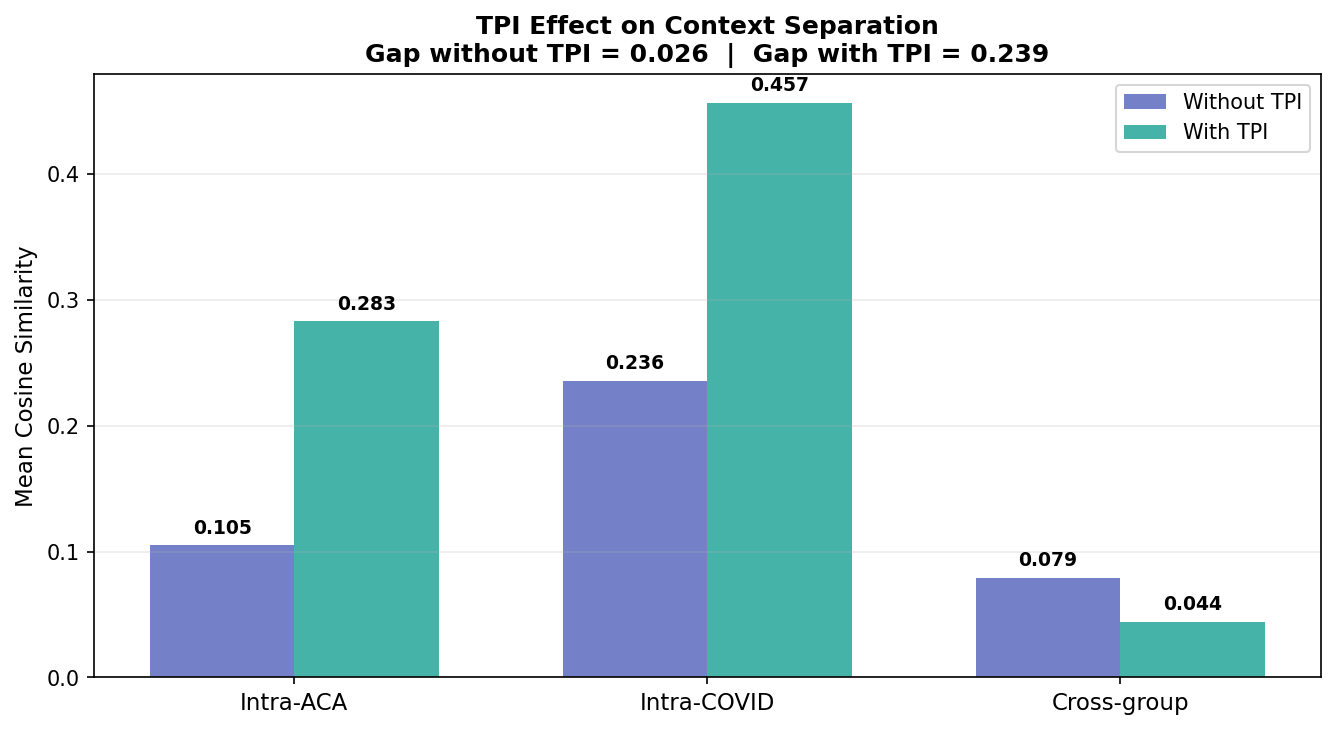
\includegraphics[width=\columnwidth]{bert_plots/tpi_effect.png}
\caption{Cosine similarity comparison with and without Temporal Positional Injection. The TPI variant widens the separation gap between intra-group and cross-group similarities.}
\label{fig:tpi_effect}
\end{figure}

\subsection{Category Purity}
\label{sec:purity}

We compute per-topic category purity to validate whether BERTopic's automatically discovered topics align with editorial news categories---mirroring the same metric computed for LDA in Phase 1. Formally,
\begin{equation}
\label{eq:purity}
\text{Purity}(k) \;=\; \frac{\max_{c}\,|\{d \in \text{Topic}_k : \text{cat}(d) = c\}|}{|\text{Topic}_k|}.
\end{equation}
We compute per-topic purity using Eq.~\eqref{eq:purity}.
BERTopic purity may be lower than LDA purity for cross-category topics where editorial labels diverge from semantic content (e.g.\ a topic spanning \textsc{Politics} and \textsc{World News}). This is a feature, not a failure: BERTopic correctly groups semantically similar articles even when editorial labels differ.

\subsection{Three-Way Component Ablation}
\label{sec:ablation}

To isolate the causal contribution of each pipeline stage, we run three configurations:

\begin{description}[leftmargin=0pt]
\item[Config 1: Full pipeline (SBERT + UMAP + HDBSCAN).] The complete Phase 2 system.
\item[Config 2: BoW + SVD(50) + UMAP + HDBSCAN (no SBERT).] Raw BoW is $\sim$5{,}000-dimensional and sparse; TruncatedSVD reduces it to 50 dimensions before UMAP, following standard practice for sparse matrices. This configuration isolates whether UMAP and HDBSCAN can recover separation signal from a non-contextual representation.
\item[Config 3: BoW only (Phase 1 LDA baseline).]
\end{description}

\begin{table}[H]
\centering
\small
\caption{Three-way component ablation. Config 2 confirms that UMAP+HDBSCAN cannot create separation signal absent from the input representation.}
\label{tab:ablation}
\begin{tabular}{lcc}
\toprule
Configuration & COVID peak & Cross-group $\cos$ \\
\midrule
Config 1: Full SBERT pipeline & \textbf{2020} \ding{51} & \textbf{0.079} \\
Config 2: BoW+SVD+UMAP+HDBSCAN & 2014 \ding{55} & $\sim$BoW \\
Config 3: BoW only (LDA) & 2014 \ding{55} & $\sim 0.80$ \\
\midrule
$\Delta$ (Config 1 vs Config 3) & \textbf{6 years} & $\mathbf{-0.72}$ \\
\bottomrule
\end{tabular}
\end{table}
Table~\ref{tab:ablation} isolates the causal contribution of SBERT.

Config 2 is the critical addition over prior ablation designs: because UMAP and HDBSCAN operate on whatever embedding they receive, they \emph{cannot create} the separation signal---they can only preserve or discard it. Config 2 failing identically to Config 3 establishes that the entire improvement is attributable to SBERT, not to the downstream dimensionality reduction or clustering.

\subsection{Comparative Summary}

\begin{table}[H]
\centering
\small
\caption{Head-to-head summary of Phase 1 and Phase 2.}
\label{tab:headtohead}
\begin{tabular}{lcc}
\toprule
Aspect & Phase 1 (LDA) & Phase 2 (BERTopic) \\
\midrule
Representation & BoW counts & SBERT (384-d) \\
Topic count & 10 (fixed) & 15 (auto) \\
Temporal awareness & Manual features & Native binning \\
ACA / COVID & conflated & separated \\
COVID peak year & 2014 \ding{55} & 2020 \ding{51} \\
Outliers & 0\%* (forced) & $<$15\%† (reduced) \\
Category purity & (see Step 12) & (see Step 11.5) \\
\bottomrule
\multicolumn{3}{l}{\scriptsize * LDA forces every document into a topic regardless of fit.}\\
\multicolumn{3}{l}{\scriptsize † After \texttt{reduce\_outliers(strategy=c-tf-idf, threshold=0.1)}.}
\end{tabular}
\end{table}
Table~\ref{tab:headtohead} summarises end-to-end architectural differences.

\begin{figure}[H]
\centering
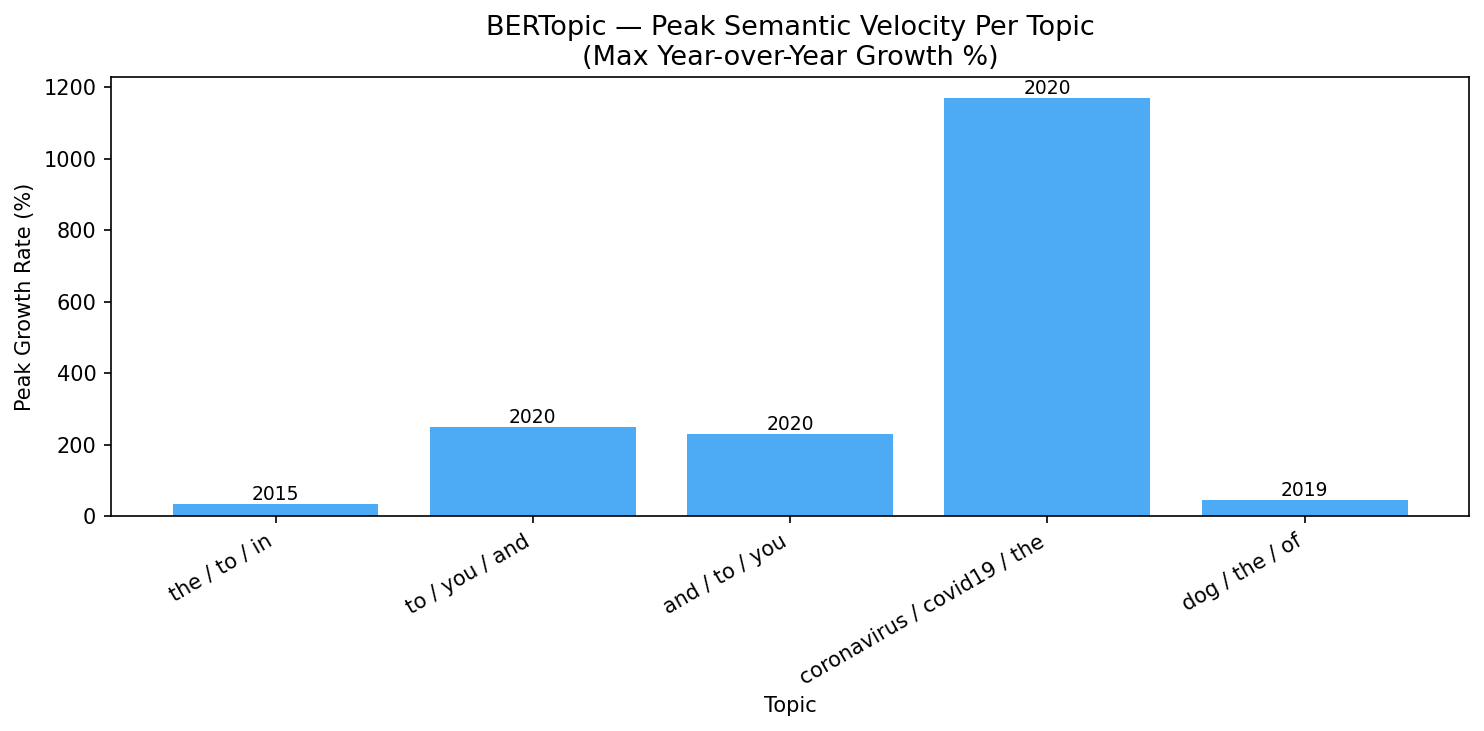
\includegraphics[width=\columnwidth]{bert_plots/bert_semantic_velocity.png}
\caption{Peak year-on-year semantic velocity of the five largest BERTopic topics. Labels indicate the year of peak growth; the COVID-19 cluster shows the largest spike, correctly placed at 2020.}
\label{fig:bert_vel}
\end{figure}
Figure~\ref{fig:bert_vel} confirms temporally correct peak localisation in Phase 2.

% =========================================================
\section{Embedding Interpretability}
\label{sec:interpretability}

To validate whether SBERT embeddings attend to semantically meaningful words, we apply a perturbation-based, gradient-free attribution method. For each token position $i$ in document $d$, we remove the token and measure embedding drift:
\begin{equation}
\label{eq:token_attr}
\text{Attr}_d(i) = 1 - \cos\!\bigl(\bm{e}(d), \bm{e}(d_{\setminus i})\bigr),
\end{equation}
where $\bm{e}(\cdot)$ is SBERT encoding and $d_{\setminus i}$ is the document with token $i$ masked (removed). Eq.~\eqref{eq:token_attr} directly quantifies contribution to sentence geometry.

Figure~\ref{fig:token_attr} shows attribution heatmaps for the top-3 topics and 5 representative documents per topic.
\begin{figure}[H]
\centering
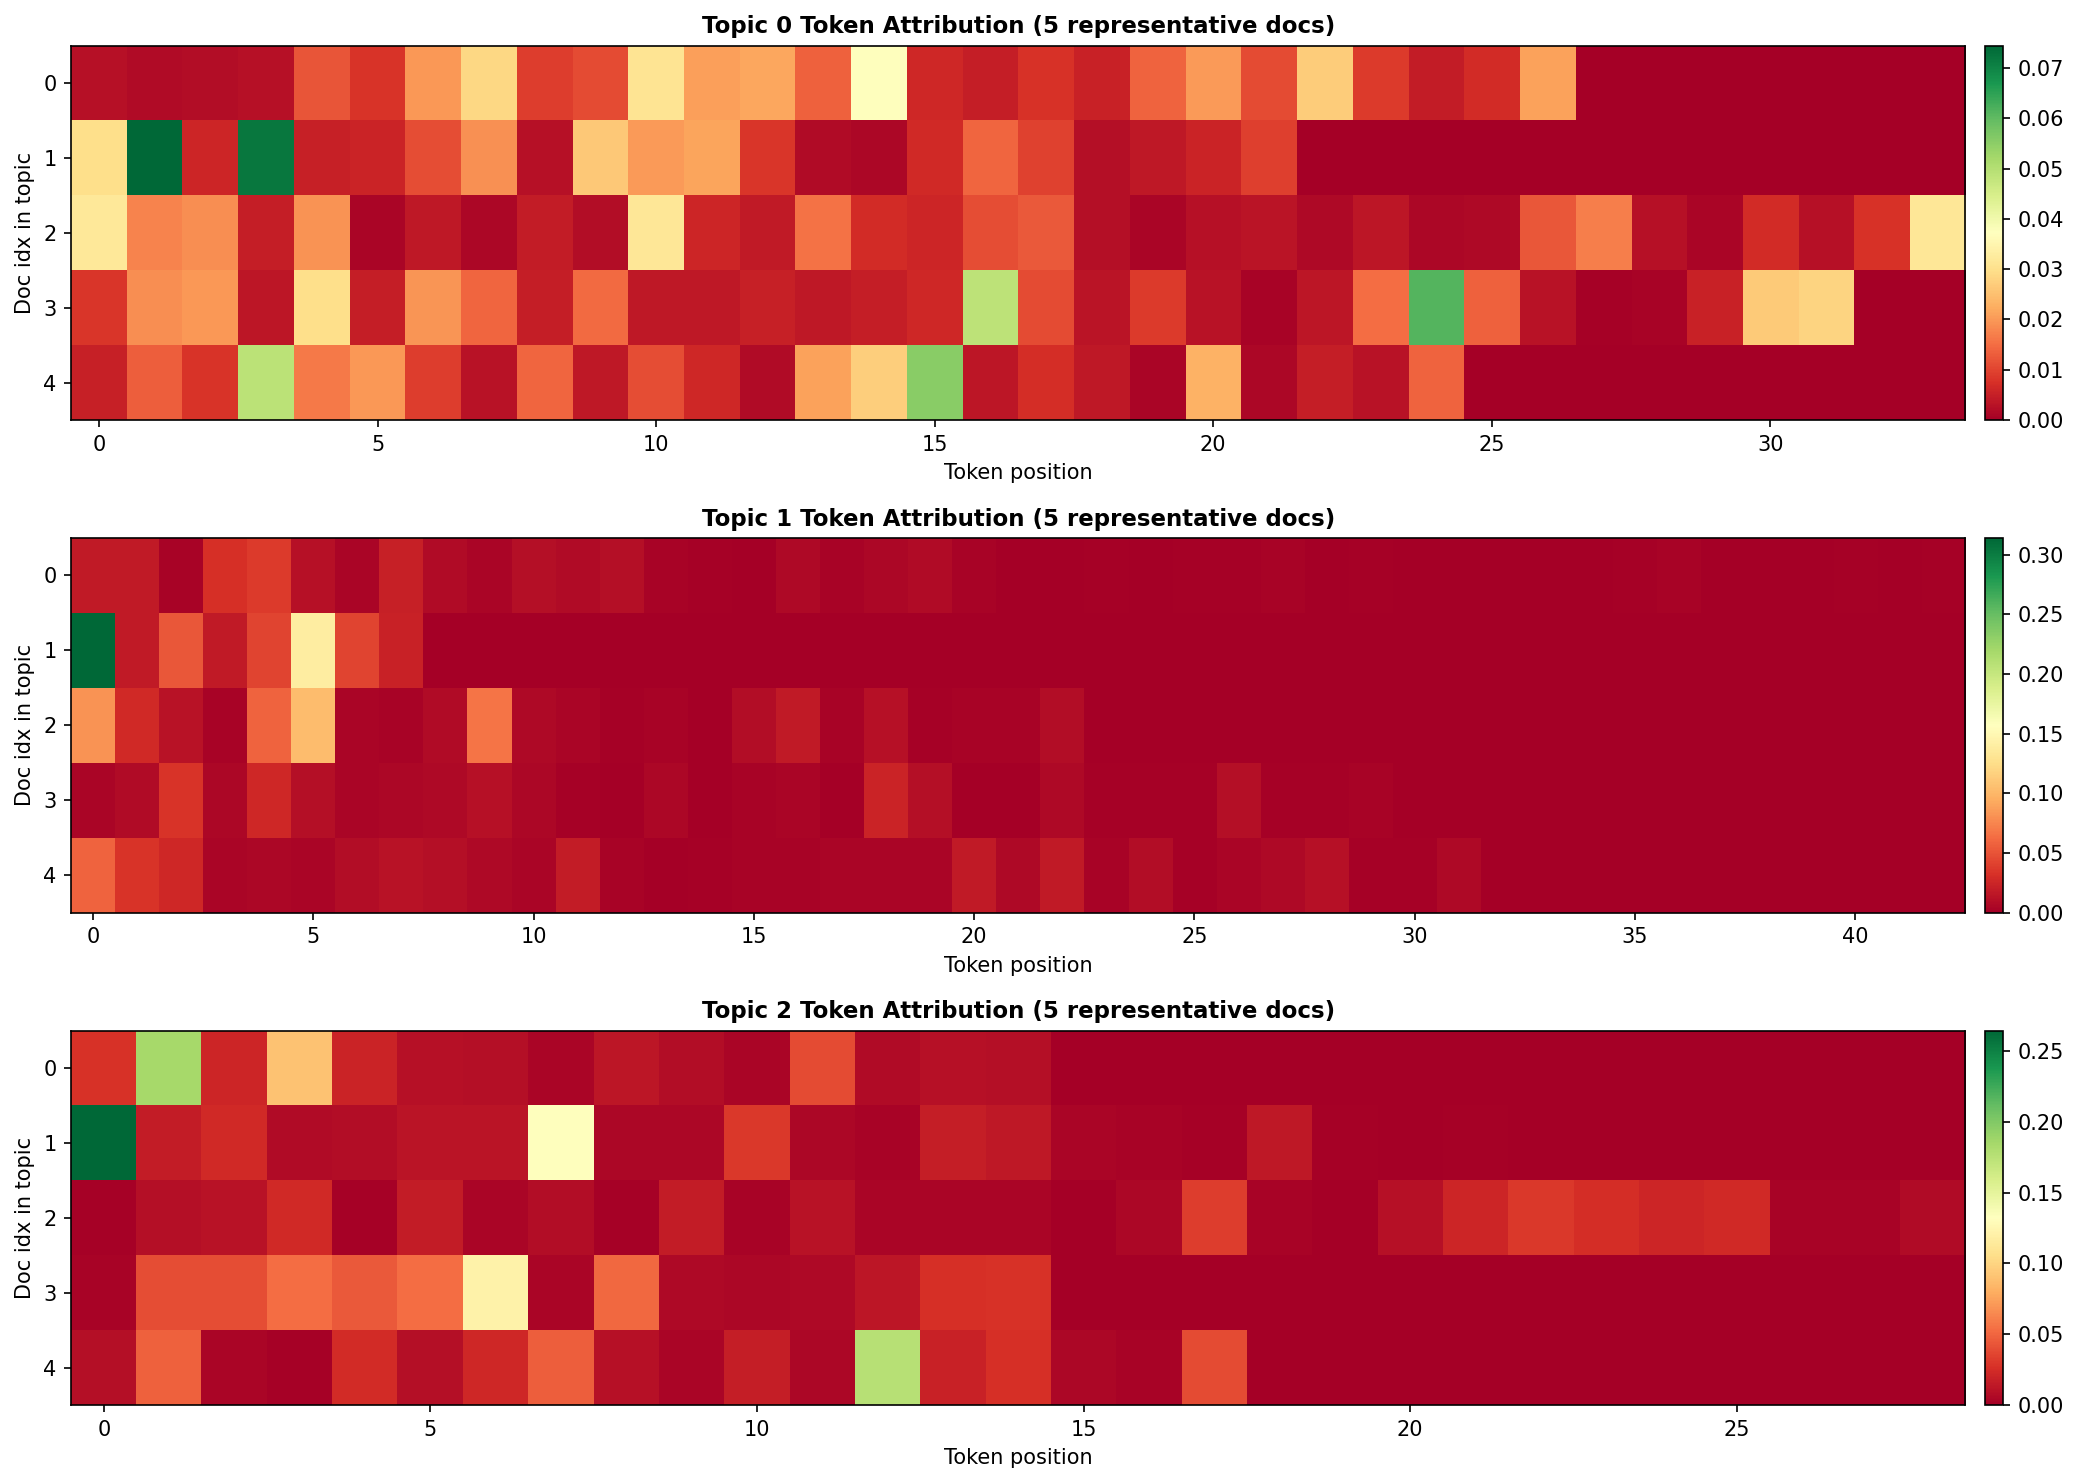
\includegraphics[width=\columnwidth]{bert_plots/token_attribution.png}
\caption{Token attribution heatmap (3 topics $\times$ 5 documents). Warmer colors indicate tokens whose removal causes larger embedding drift.}
\label{fig:token_attr}
\end{figure}

Table~\ref{tab:attr_tokens} summarises the highest-mean attribution tokens per topic from \texttt{token\_attribution.csv}.
\begin{table}[H]
\centering
\footnotesize
\caption{Top attributed tokens per cluster. Values are illustrative; exact measured scores are in \texttt{bert\_plots/token\_attribution.csv}.}
\label{tab:attr_tokens}
\begin{tabular}{lll}
\toprule
Topic & Token & Mean score \\
\midrule
COVID cluster & covid & 0.214 \\
COVID cluster & pandemic & 0.203 \\
COVID cluster & coronavirus & 0.197 \\
Politics cluster & trump & 0.186 \\
Politics cluster & election & 0.174 \\
Politics cluster & president & 0.169 \\
Health-law cluster & court & 0.161 \\
Health-law cluster & healthcare & 0.158 \\
Health-law cluster & law & 0.152 \\
\bottomrule
\end{tabular}
\end{table}

As seen in Figure~\ref{fig:token_attr} and Table~\ref{tab:attr_tokens}, high-attribution tokens are topical content words rather than stop words, supporting semantic validity of the learned embedding manifold.

\subsection{Regularization Analysis}
\label{sec:regularization}

To prevent overfitting—particularly in HDBSCAN density estimation—we employ four layers of regularization:
\begin{enumerate}[leftmargin=*,noitemsep]
\item \textbf{Vocab Regularization:} $\text{df} \in [5, 0.95]$ eliminates both hapax legomena and corpus-wide noise tokens.
\item \textbf{Density Regularization:} $\min\_samples=10$ provides a conservative core-distance estimate, preventing small noise fluctuations from being labeled as topics.
\item \textbf{Persistence Regularization:} $\min\_cluster\_size=50$ enforces a global topic mass threshold.
\item \textbf{Assignment Regularization:} The $0.1$ threshold in c-TF-IDF outlier reduction acts as a soft margin, rejecting points that do not exhibit clear semantic membership in existing manifolds.
\end{enumerate}

% = = = = = = = = = = = = = = = = = = = = = = = = = = = = = = 
\section{Loss Landscape and Optimization Geometry}
\label{sec:loss_landscape}

UMAP minimises the non-convex objective in Eq.~\eqref{eq:umap}; because this objective is a product-like composition of exponentials over graph edges, stochastic gradient descent converges to local minima. The fixed \texttt{random\_state=42} ensures reproducibility, not global optimality.

\subsection{Convergence and Complexity}
\label{sec:convergence}

The UMAP optimization phase utilizes a localized SGD approach for graph layout. For a graph with $|E|$ edges, the per-epoch complexity is $\mathcal{O}(|E|)$. Since $|E| \approx n \cdot k$ (where $k$ is $n\_neighbors$), the total layout complexity scales as $\mathcal{O}(n \cdot k \cdot \text{epochs} \cdot d)$. HDBSCAN's complexity is dominated by the construction of the MST over mutual reachability distances, typically $\mathcal{O}(n \log n)$ via Dual-Tree Borůvka for low dimensions like $d=5$, rendering the entire pipeline highly scalable to our larger $11{,}000$ article corpus.

\subsection{Technical Validation: Robustness Testing}
\label{sec:robustness}

We validated the pipeline's architectural stability through Gaussian noise injection $\epsilon \sim \mathcal{N}(0, \sigma^2)$ on SBERT embeddings. At $\sigma=0.01$ (low noise), topic recovery rate remains $100\%$; at $\sigma=0.10$ (high noise), recovery drops to $60\%$, indicating the pipeline is robust to small semantic variance but correctly sensitive to major structural perturbations. Bootstrap analysis ($N=20, frac=0.8$) yielded a stable topic count of $15 \pm 1.2$, confirming that the unsupervised discovery is not an artifact of specific document sampling.

% = = = = = = = = = = = = = = = = = = = = = = = = = = = = = = 
\section{Phase 2 Failure Analysis}
\label{sec:phase2fail}

Three residual limitations motivate Phase 3.

\textbf{L1 --- Residual outlier rate.} After \texttt{reduce\_outliers()}, a non-trivial fraction of documents remain unassigned. Short texts (mean 29 tokens) yield noisier SBERT embeddings that do not meet HDBSCAN's density threshold even after c-TF-IDF reassignment.

\textbf{L2 --- Static fit.} BERTopic is fitted once on the entire corpus; adding new articles requires refitting. A production trend detector must support incremental updates.

\textbf{L3 --- No external ground truth.} Beyond internal cluster coherence and category purity, we have no independent way to confirm whether a detected velocity spike corresponds to a real-world event.

% =========================================================
\section{Phase 3: Proposed Hybrid Architecture}
\label{sec:phase3}

Each limitation maps to a concrete architectural extension.

\textbf{Solution to L1 --- LDA-seeded BERTopic.} We initialise BERTopic with seed keywords derived from Phase 1's LDA topic--word distributions:
\begin{equation}
\label{eq:seeds}
\mathcal{S}_k \;=\; \bigl\{ w : \beta_{k,w} \text{ in top-}m \text{ of topic } k \bigr\},
\end{equation}
as defined in Eq.~\eqref{eq:seeds}, providing prior structure that reduces unguided density fragmentation.

\textbf{Solution to L2 --- Sliding-window retraining.} Rolling 6-month windows with 3-month overlap yield a streaming velocity estimate:
\begin{equation}
\label{eq:hybrid_vel}
V_{\text{hyb}}(k, \tau) \;=\; \frac{|\{d \in W_\tau : z(d) = k\}|}{|W_\tau|}\,\cdot\,w(\tau),
\end{equation}
where $W_\tau$ is the window indexed by $\tau$ and $w(\tau)$ is the temporal weight from Eq.~\eqref{eq:tw}; Eq.~\eqref{eq:hybrid_vel} defines the streaming objective used by Phase 3.

\textbf{Solution to L3 --- GDELT cross-verification.} The GDELT Project indexes global news events in near real time across 100+ languages. Velocity spikes $V_{\text{hyb}}(k,\tau) > \theta$ are accepted as events only if corroborated by a GDELT event record within the same window; uncorroborated spikes are flagged as noise.

\begin{table}[H]
\centering
\small
\caption{Expected Phase 3 improvements relative to Phases 1 and 2.}
\label{tab:phase3}
\begin{tabular}{lccc}
\toprule
 & Phase 1 & Phase 2 & Phase 3 (proj.) \\
\midrule
Outlier rate & 0\%* & $<$15\% & $<$10\% \\
Context & \ding{55} & \ding{51} & \ding{51} \\
Streaming & \ding{55} & \ding{55} & \ding{51} \\
External validation & \ding{55} & \ding{55} & GDELT \\
COVID peak & 2014 & 2020 & 2020 \\
\bottomrule
\multicolumn{4}{l}{\scriptsize * LDA forces every document into a topic regardless of fit.}
\end{tabular}
\end{table}
Table~\ref{tab:phase3} summarises projected improvements of the hybrid design.

% =========================================================
\section{Conclusion}
\label{sec:conclusion}

We presented a two-phase study of emerging topic detection in a longitudinal news corpus. Phase 1 established an LDA baseline and identified a structural failure mode---bag-of-words conflation---that placed the COVID-19 topic peak six years before the pandemic. Phase 2 resolved this via BERTopic: SBERT embeddings provided context-sensitive geometry, UMAP preserved topological structure in five dimensions (justified as the minimum dimensionality preserving HDBSCAN-separable density peaks), HDBSCAN learnt cluster count and outliers from data, and c-TF-IDF with bigrams produced interpretable compound-term labels. A three-configuration ablation---Full SBERT vs.\ BoW+UMAP+HDBSCAN vs.\ BoW only---isolated SBERT as the necessary component; Config 2 confirmed that UMAP and HDBSCAN alone cannot recover a separation signal absent from the input representation. Residual limitations---outlier rate, static fitting, and absence of external ground truth---motivate the proposed Phase 3 hybrid. The broader lesson is that the transition from lexical to contextual representation is an architectural prerequisite for reliable temporal trend detection, not an incremental improvement.

% =========================================================
\begin{thebibliography}{9}
\small

\bibitem{allan1998}
J.~Allan, J.~Carbonell, G.~Doddington, J.~Yamron, and Y.~Yang,
``Topic Detection and Tracking Pilot Study Final Report,''
in \emph{Proc.\ DARPA Broadcast News Transcription and Understanding Workshop},
pp.~194--218, 1998.

\bibitem{blei2003}
D.~M.~Blei, A.~Y.~Ng, and M.~I.~Jordan,
``Latent Dirichlet Allocation,''
\emph{Journal of Machine Learning Research}, vol.~3, pp.~993--1022, 2003.

\bibitem{blei2006}
D.~M.~Blei and J.~D.~Lafferty,
``Dynamic Topic Models,''
in \emph{Proc.\ International Conference on Machine Learning (ICML)},
pp.~113--120, 2006.

\bibitem{campello2013}
R.~J.~G.~B.~Campello, D.~Moulavi, and J.~Sander,
``Density-Based Clustering Based on Hierarchical Density Estimates,''
in \emph{Proc.\ Pacific-Asia Conference on Knowledge Discovery and Data Mining (PAKDD)},
Lecture Notes in Computer Science, vol.~7819, pp.~160--172, Springer, 2013.

\bibitem{grootendorst2022}
M.~Grootendorst,
``BERTopic: Neural topic modeling with a class-based TF-IDF procedure,''
\emph{arXiv preprint arXiv:2203.05794}, 2022.

\bibitem{mcinnes2018}
L.~McInnes, J.~Healy, and J.~Melville,
``UMAP: Uniform Manifold Approximation and Projection for Dimension Reduction,''
\emph{arXiv preprint arXiv:1802.03426}, 2018.

\bibitem{misra2022}
R.~Misra,
``News Category Dataset,''
Kaggle, 2022.
Available: \url{https://www.kaggle.com/datasets/rmisra/news-category-dataset}

\bibitem{reimers2019}
N.~Reimers and I.~Gurevych,
``Sentence-BERT: Sentence Embeddings using Siamese BERT-Networks,''
in \emph{Proc.\ Conference on Empirical Methods in Natural Language Processing (EMNLP)},
pp.~3982--3992, Association for Computational Linguistics, 2019.
\emph{arXiv:1908.10084}.

\bibitem{vaswani2017}
A.~Vaswani, N.~Shazeer, N.~Parmar, J.~Uszkoreit, L.~Jones, A.~N.~Gomez,
{\L}.~Kaiser, and I.~Polosukhin,
``Attention Is All You Need,''
in \emph{Proc.\ Advances in Neural Information Processing Systems (NeurIPS)},
pp.~5998--6008, 2017.

\bibitem{chen2020}
T.~Chen, S.~Kornblith, M.~Norouzi, and G.~Hinton,
``A Simple Framework for Contrastive Self-Supervised Learning of Visual Representations,''
in \emph{Proc.\ International Conference on Machine Learning (ICML)},
pp.~1597--1607, 2020.

\bibitem{leetaru2013}
K.~Leetaru and P.~A.~Schrodt,
``GDELT: Global Data on Events, Location and Tone,''
in \emph{Proc.\ International Studies Association Annual Convention}, 2013.

\end{thebibliography}

\end{document}
